\chapter{Imperative und deklarative Modellierung für SE-Prozessmodelle}\label{sec:chapter6}
In diesem Kapitel wird der Vergleich zwischen imperativer und deklarativer Modellierung für SE-Prozessmodelle durchgeführt. Als Erstes wird dieser Vergleich in Kapitel 6.1 für das SE-Prozessmodelle Scrum durchgeführt. Hierfür wird zunächst in Kapitel 6.1 das der Modellierung zugrunde liegende Modell, das SE-Prozessmodell Scrum, vorgestellt und in Kapitel 6.1.1 für die Modellierung analysiert. Danach erfolgt in Kapitel 6.1.2 die imperative Modellierung von in der Prozessmodellierungssprache BPMN und anschließend die deklarative Modellierung in der Prozessmodellierungssprache ConDec in Kapitel 6.1.3. Danach erfolgt  in Kapitel 6.1.4 der Vergleich zwischen den beiden Modellen.\newline
Der zweite SE-Prozess, welcher in diesem Kapitel in imperativer und deklarativer Prozessmodellierungssprache verglichen werden soll, ist der Open Unified Process (Open Up). Auch hier erfolgt zunächst eine kurze Einführung in den Open Up in Kapitel 6.2, bevor dieser in Kapitel 6.2.1 analysiert wird, damit er in den Kapiteln 6.2.2 und 6.2.3 in imperativer, bzw. deklarativer Prozessmodellierungssprache modelliert werden kann. Hiernach erfolgt in Kapitel 6.2.4 der Vergleich zwischen den Prozessmodellen.\newline
Zuletzt wird noch das V-Modell XT modelliert und verglichen. Eine Einführung in das V-Modell XT erfolgt in Kapitel 6.3. In Kapitel 6.3.1 wird dieses als Vorbereitung für die Modellierung analysiert und in den Kapiteln 6.3.2 und 6.3.3 in imperativer und deklarativer Prozessmodellierungssprache modelliert. Der Vergleich hierzu erfolgt in Kapitel 6.3.4.


\section{Scrum}\label{sec:chapter6:Imperative Modellierung}

Der Begriff Scrum stammt aus dem Artikel "The New New Product Development Game", welchen Hirotaka Takeuchi und Ikujiro Nonaka im Harvard Business Review 1986 veröffentlicht haben. Sie beschrieben einen ganzheitlichen Ansatz bei dem kleine, funktionsübergreifende Teams zusammen an einem gemeinsamen Ziel arbeiten. Dies verglichen sie mit der Scrum-Formation beim Rugby \cite{Pham2012,Takeuchi1986}. \newline
Bei Scrum handelt es sich um ein agiles Prozessmodell, welches seit Anfang 1990 für komplexe Entwicklungen verwendet wird. Agile Prozessmodelle werden den leichtgewichtigen Prozessmodellen zugeordnet \cite{Hanser2010, Lacey2012}. Einen ersten Überblick über das Scrum-Prozessmodell gibt Abbildung \ref{fig:Scrum}:

\begin{figure}[htp]
\begin{center}
  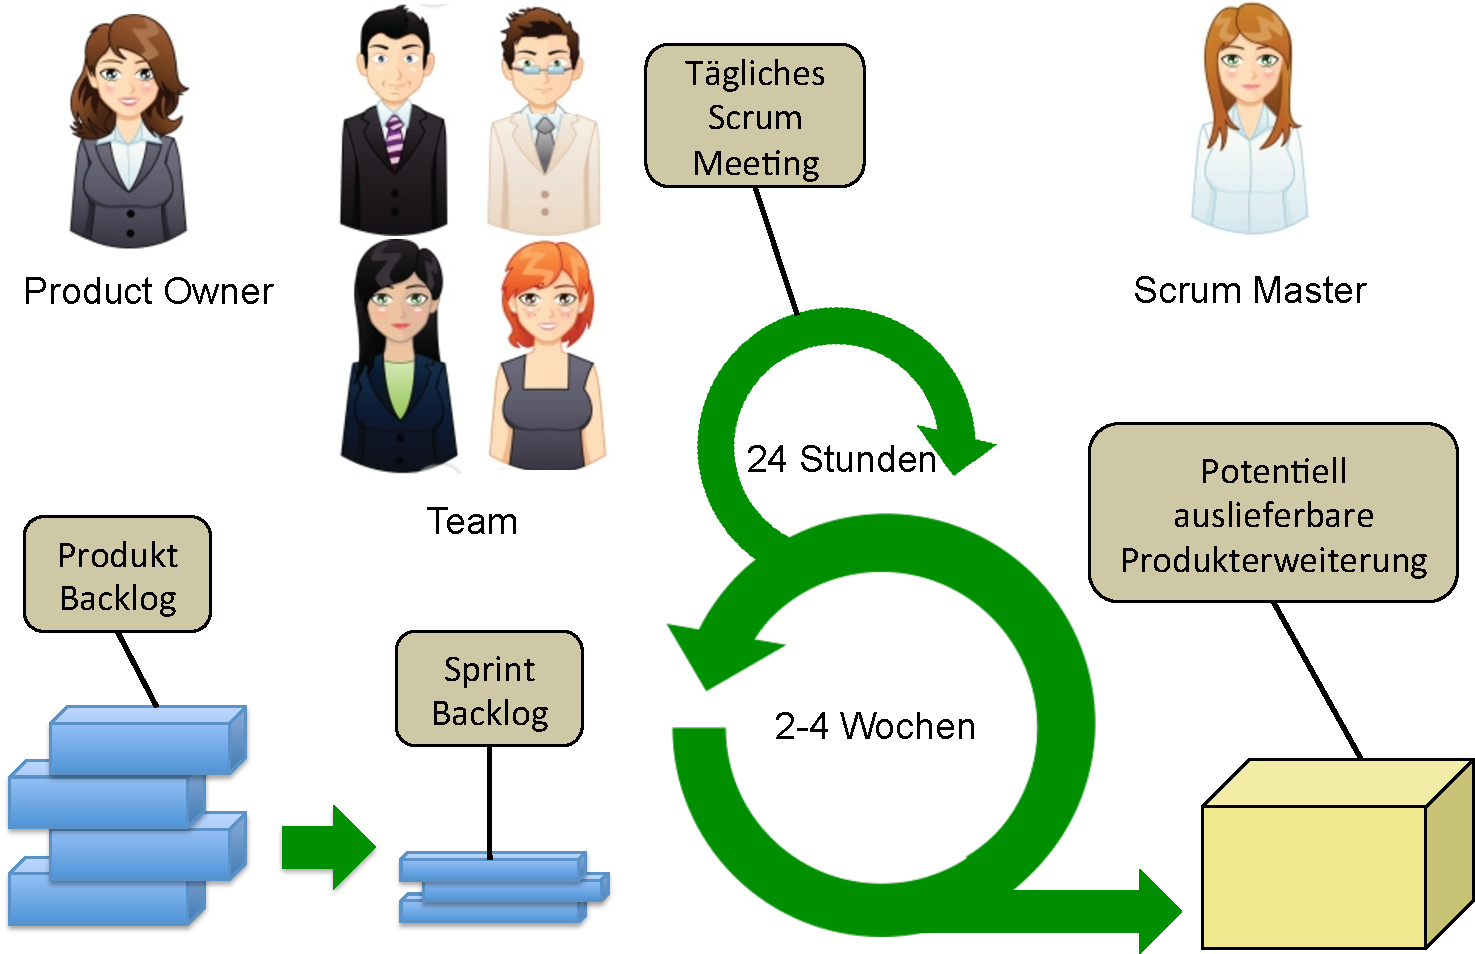
\includegraphics[scale=0.6]{Scrum} %pdf, jpg, png...
  \caption{Scrum Überblick nach \cite{scrum2008}}
  \label{fig:Scrum}
\end{center}
\end{figure}

Der genaue Ablauf im Scrum Prozessmodell wird nachfolgend genau analysiert.

\subsection{Analyse Scrum}


Im Scrum-Prozessmodell gibt es nur drei verschiedene Rollen: Den \textit{Product Owner}, das \textit{Team} und den \textit{Scrum Master}. Sämtliche Verantwortlichkeiten innerhalb eines Projektes werden hierbei auf diese drei Rollen aufgeteilt \cite{Schwaber2004}. \newline

Der \textit{Procuct Owner} ist verantwortlich, die Interessen aller am Projekt beteiligten Personen zu vertreten. Neben der Budgetierung des Projektes erstellt er ebenfalls Releasepläne und erstellt den Produkt-Backlog, welcher eine Liste mit funktionalen und nicht-funktionalen Anforderungen darstellt \cite{Schwaber2004, Pichler2010,Schwaber2007}. Weiterhin priorisiert er die Aufgaben, welche von den Entwicklern im Sprint erledigt werden sollen, so dass die aktuell nützlichsten Elemente die höchste Priorität haben. Er erstellt eine Liste dieser Elemente, welche \textit{Sprint-Backlog} genannt wird \cite{Henning2011, Schwaber2007,Pichler2010}. Der \textit{Procuct Owner} ist ebenfalls zuständig für das Annehmen, bzw. Ablehnen der Arbeitsergebnisse \cite{eclipseScrum}. \newline

Die \textit{Teams} bestehen bei Scrum für gewöhnlich aus fünf bis neun Mitgliedern und verwalten sich selbst. Ihre Tätigkeiten müssen erfolgreich sein, liegen aber in ihrer eigenen Verantwortung \cite{Pries2011, Wolf2011}. Alle Teammitglieder sind gemeinsam für den Erfolg eines jeden \textit{Sprints} und des gesamten Projektes verantwortlich \cite{Pichler2010}. \newline

Der \textit{Scrum-Master} ist für den gesamten Scrum-Prozess verantwortlich. Dies schließt die Vermittlung von Scrum-Inhalten (z.B. Schulungen) und die Implementation von Scrum in die Unternehmenskultur ein \cite{Pichler2010}. Er überwacht die Sprint- Tasks, um sicher zu gehen, dass der Sprint erfolgreich verläuft.\newline

Bei Scrum wird die Entwicklung in mehrere kurze Zyklen, also Iterationen eingeteilt. Eine einzelne Iteration wird bei Scrum \textit{Sprint} genannt \cite{Henning2011}. Die Dauer eines Sprints beträgt zwei bis vier Wochen. Am Ende eines jeden Sprints muss das \textit{Team} ein lauffähiges Produkt abliefern \cite{Wolf2011}. Vor jedem Sprint findet ein \textit{Sprint Planning Meeting} statt, welches sich aus zwei Teilen zusammensetzt \cite{Pichler2010}. Im ersten Teil findet eine Planung des nächsten \textit{Sprints} statt \cite{Lacey2012}. Hierfür präsentiert der \textit{Product Owner} dem \textit{Team} eine Liste der Product-Backlog-Elemente mit der aktuell höchsten Priorität \cite{Schwaber2004, Schwaber2007,Pichler2010}. Diese Liste wird \textit{Sprint-Backlog} genannt \cite{Wolf2011}. Das \textit{Team} hat die Möglichkeit Fragen bezüglich Inhalt, Zweck, Bedeutung und Absichten der \textit{Sprint-Backlog}-Elemente zu stellen. Anschließend werden die einzelnen Elemente aus dem \textit{Sprint-Backlog} in sogenannte \textit{Tasks} aufgeteilt, welche jeweils eine ideale Bearbeitungszeit von zwei bis vier Stunden haben, aber niemals länger als zwei Tage dauern sollten \cite{Wolf2011}. Das \textit{Team} kann sich die Aufgaben eigenverantwortlich aufteilen und muss sich anschließend dem \textit{Product  Owner} verpflichten, die \textit{Tasks} bis zum Abschluss des \textit{Sprints} zu erledigen \cite{Wolf2011, Keith2010,Pichler2010}.
Das  \textit{Team} trifft sich während des \textit{Sprints} täglich in einem 15-minütigen Meeting, dem \textit{täglichem Scrum-Meeting}. Hier redet das \textit{Team} über seinen Fortschritt und eventuelle Probleme bei ihrer Arbeit \cite{Keith2010}. Hier muss jedes Teammitglied die nachfolgenden drei Fragen beantworten       \cite{Wolf2011}:
   \begin{enumerate}
      \item Was habe ich seit gestern erreicht?
      \item Was werde ich heute erreichen?
      \item Was blockiert mich?
      \end {enumerate}
      
\subsection{Imperative Modellierung Scrum}

\begin{figure}[htp]
\begin{center}
  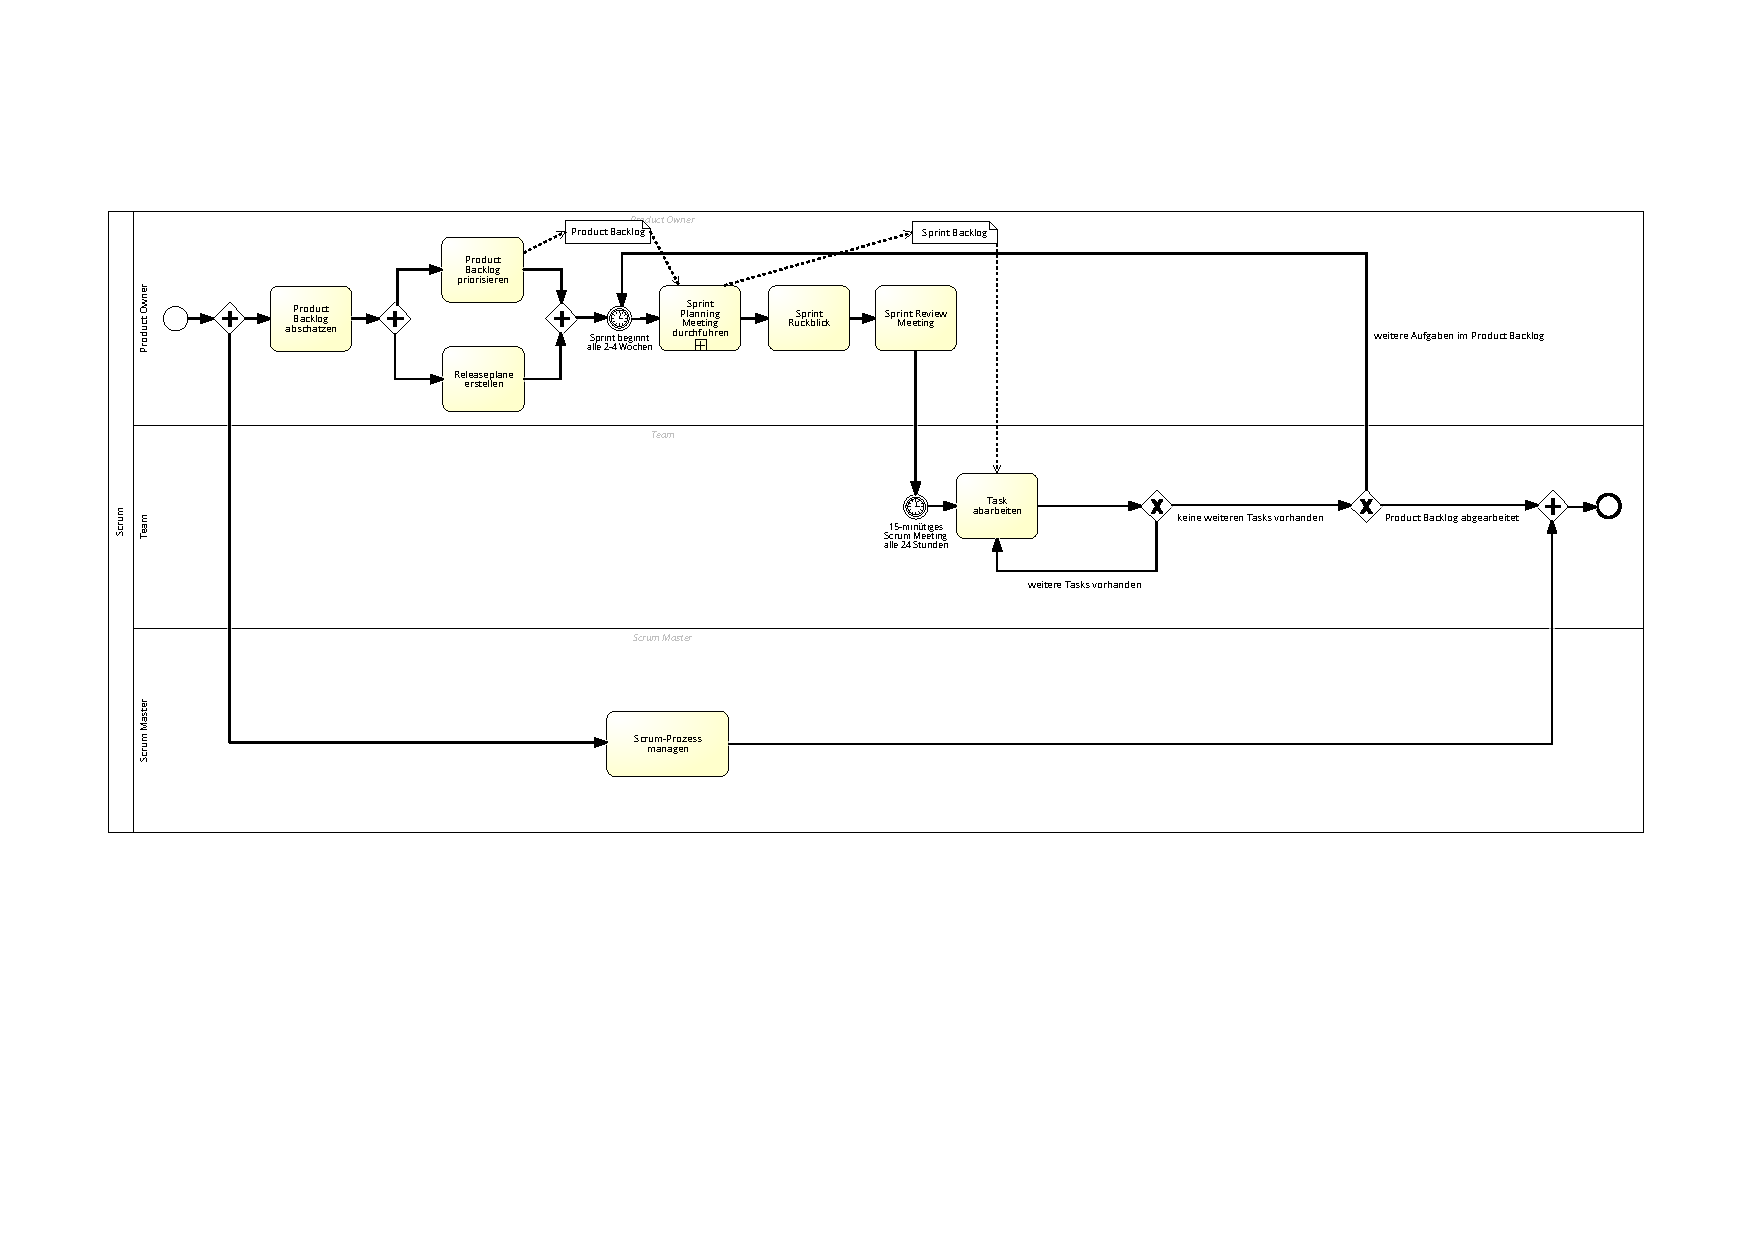
\includegraphics[width=\textwidth]{ScrumImperativ} %pdf, jpg, png...
  \caption{Imperative Modellierung Scrum}
  \label{fig:ScrumImperativ}
\end{center}
\end{figure}

\begin{figure}[htp]
\begin{center}
  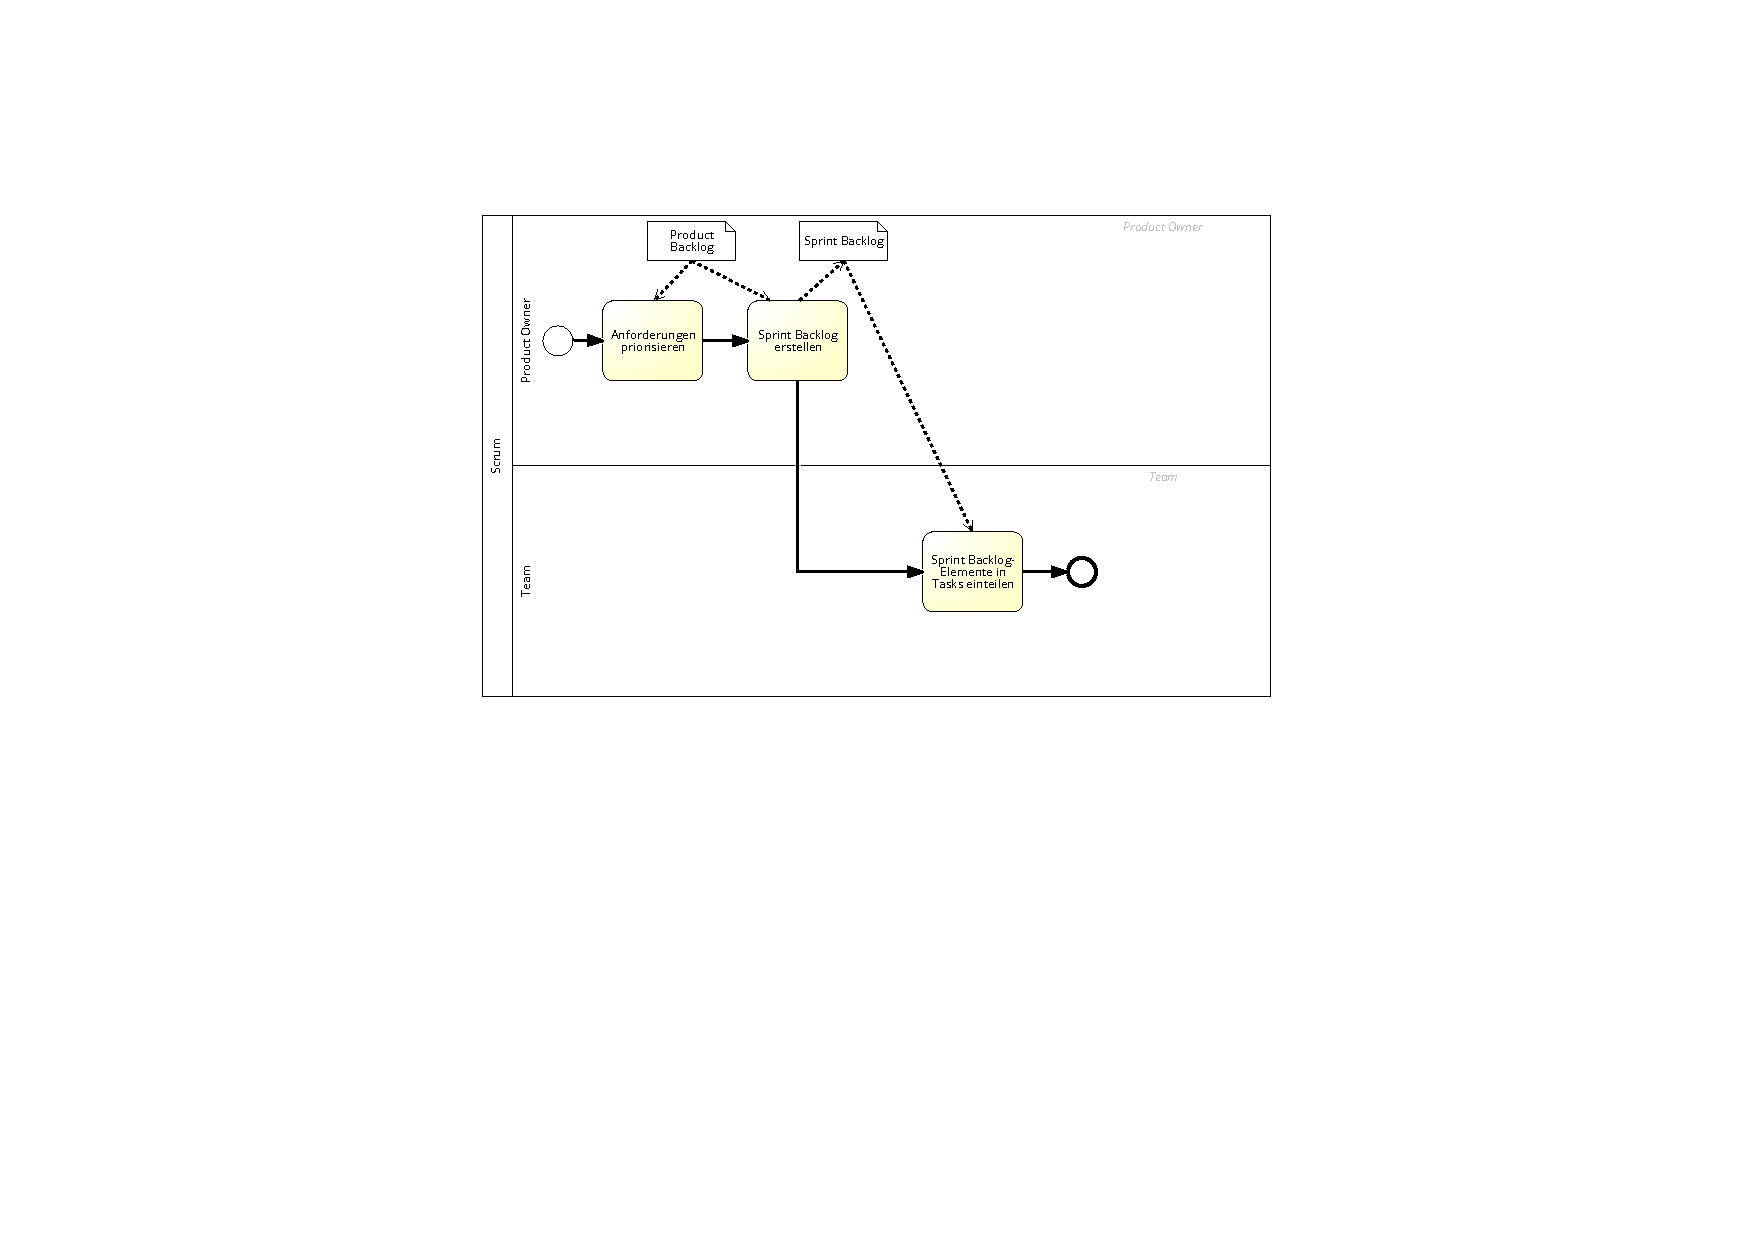
\includegraphics[width=\textwidth]{ScrumImperativUnter} %pdf, jpg, png...
  \caption{Imperative Modellierung Scrum Unterprozess}
  \label{fig:ScrumImperativUnter}
\end{center}
\end{figure}

\subsection{Deklarative Modellierung Scrum}

\begin{figure}[htp]
\begin{center}
  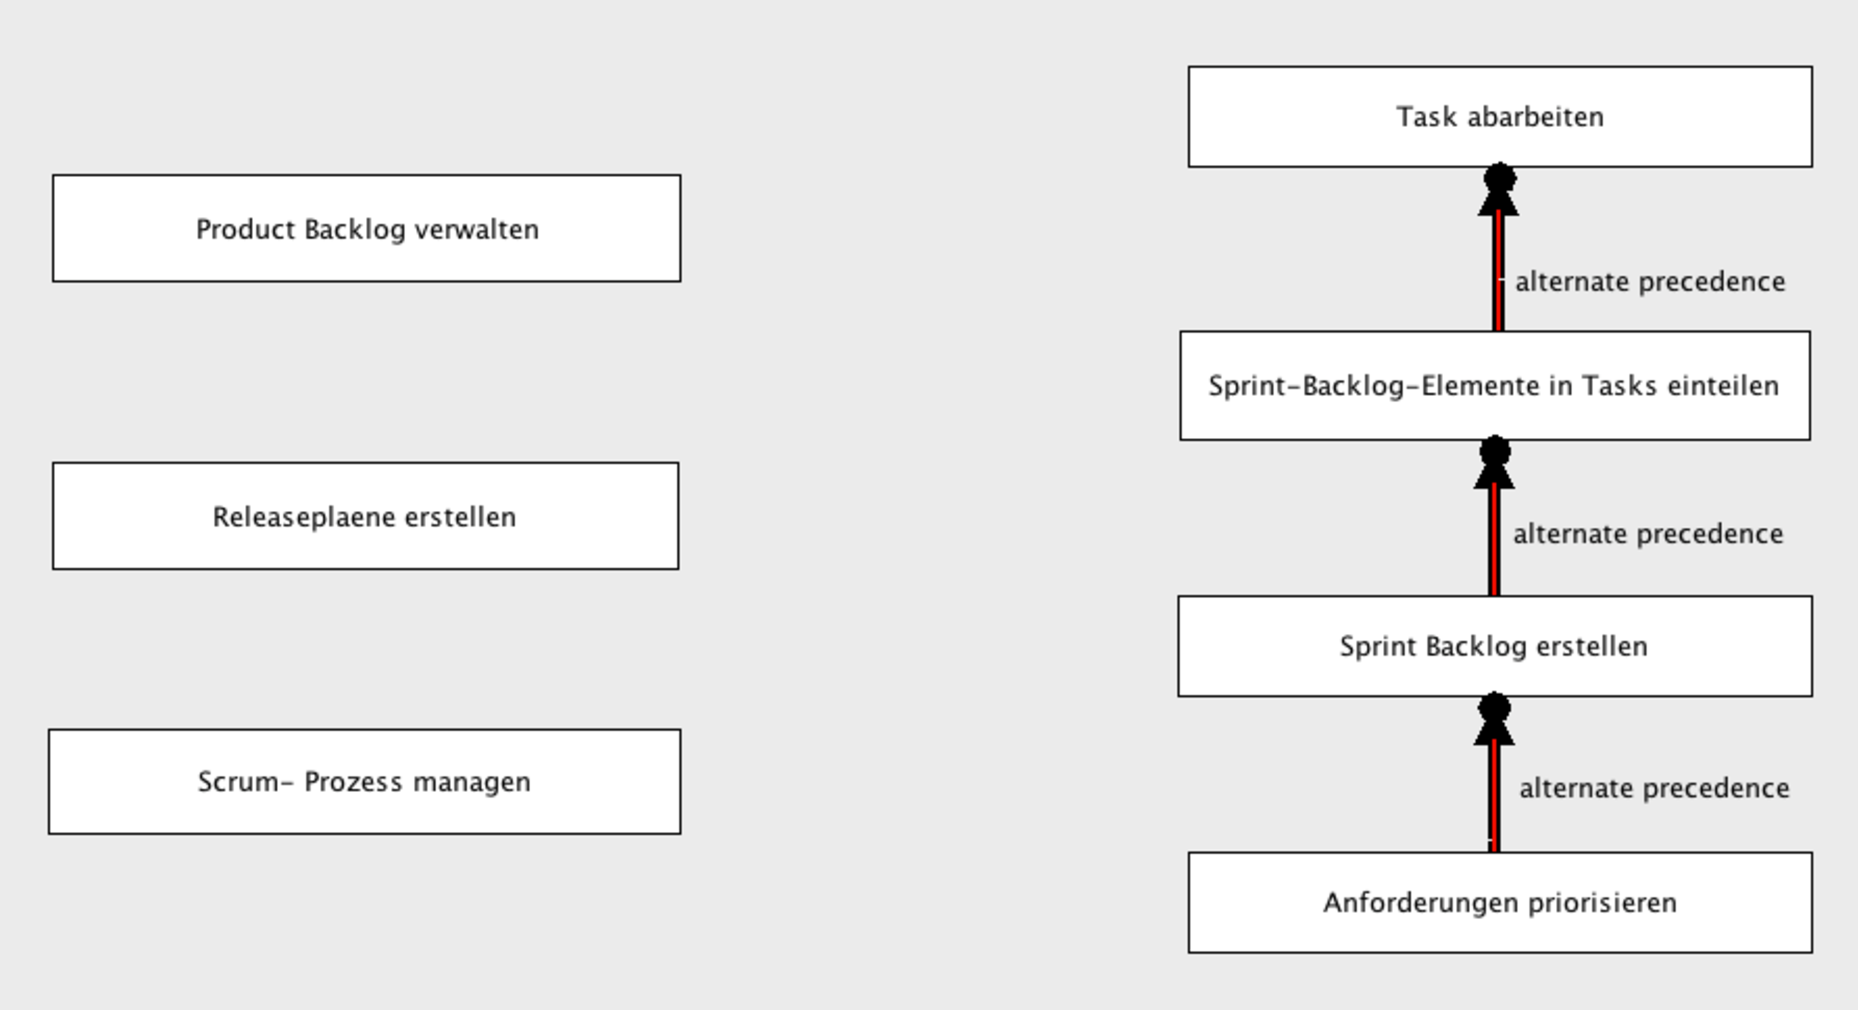
\includegraphics[width=\textwidth]{ScrumDeklarativ} %pdf, jpg, png...
  \caption{Deklarative Modellierung Scrum}
  \label{fig:ScrumDeklarativ}
\end{center}
\end{figure}

\subsection{Vergleich}



\section{Open Unified Process (Open Up)}


Der Open Unified Process, kurz Open Up ist eine frei zugängliche Variante des Rational Unified Process, welcher ein sehr bekannter Entwicklungsprozess ist \cite{hauber2010}.  Er ist Teil des Eclipse Process Frameworks. Open Up ist ein iterativer, inkrementeller und minimaler Prozess, aber dennoch vollständig und erweiterbar \cite{Gau2006, Basem2010}. Der Prozess ist minimal gehalten, da er nur die wesentlichen Inhalte einbezieht. Trotzdem ist er vollständig, da er als Prozess benutzt werden kann, um ein Softwaresystem zu entwickeln. Er ist außerdem auch erweiterbar, da er als Grundlage herangezogen werden kann und mit weiteren Prozessfragmenten aufgestockt und nach Belieben zugeschnitten werden kann \cite{Wang2007}. Das Konzept des Open Up ist es den Prozess zu vergrößern, sich aber auf das Minimum, welches für das Projekt benötigt wird zu beschränken, anstatt zu versuchen große, überladene Prozesse zu verstehen und diese dann zu verkleinern \cite{ambler2012}.  \newline



Open Up ist auf kleine Teams ausgerichtet, bei welchen bei der Zusammenarbeit räumliche Nähe besteht. Die Teammitglieder haben hierbei die Freiheit, ihre eigenen Entscheidungen bezüglich ihren aktuellen Aufgaben und Prioritäten zu treffen, um die Anforderungen der Stakeholder zu erfüllen. Das Team trifft sich täglich, um über den aktuellen Status zu reden \cite{OpenUPProcess}.\newline
Es werden Rollen, Aufgaben, Artefakte und Ebenen in Open Up definiert. Dies soll ermöglichen, dass verschiedene Sichten, die sich in ihrem Detaillierungsgrad unterscheiden auf das Projekt möglich sind \cite{freudenreichevaluierung}. Einen ersten Überblick über Open Up gibt Abbildung \ref{fig:openup}.


\begin{figure}[htp]
\begin{center}
  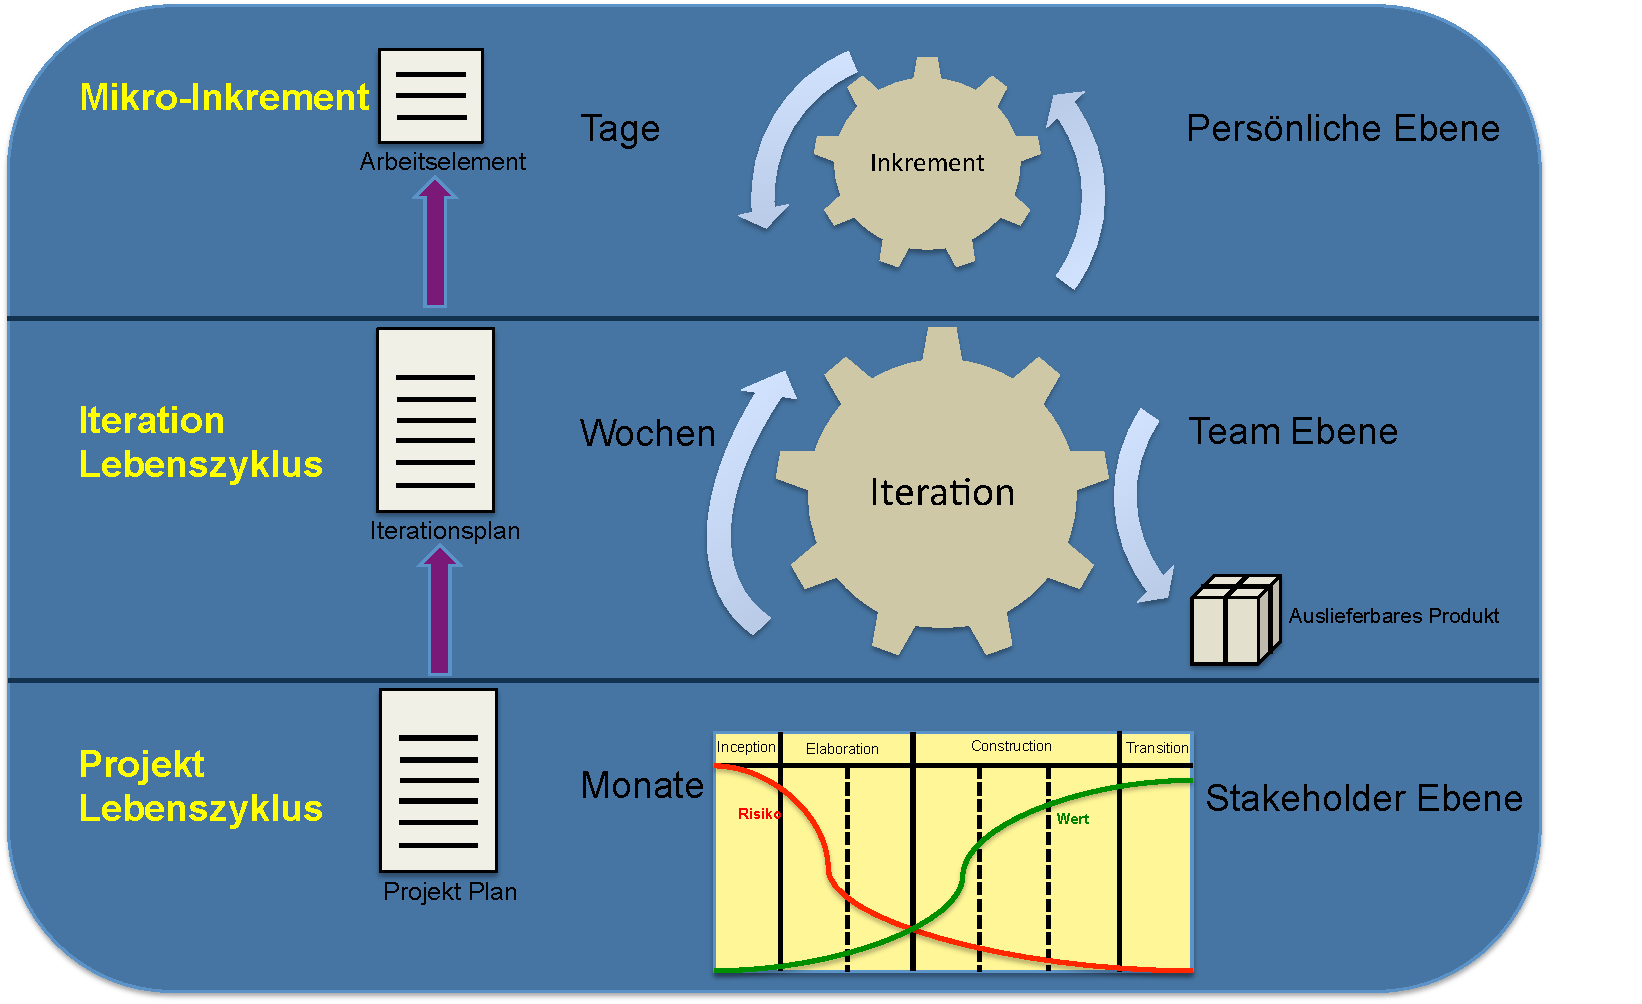
\includegraphics[width=\linewidth]{openup} %pdf, jpg, png...
  \caption{Open Up Überblick nach \cite{eclipseopenup}}
  \label{fig:openup}
\end{center}
\end{figure}

Der Open Up wird im Folgenden genauestens analysiert.

\subsection{Analyse Open Up}


Auf der persönlichen Ebene teilen sich die Teammitglieder ihre Arbeit in \textit{Mikro-Inkremente} ein. Diese stellen das Ergebnis von Stunden, bzw. wenigen Tagen Arbeit dar. Die Arbeit entwickelt sich somit ein Mikro-Inkrement weiter und der Fortschritt kann Tag für Tag nachvollzogen werden. Die Teammitglieder teilen ihre Fortschritte täglich miteinander, was die Arbeitstransparenz und das Vertrauen erhöht und die Teamarbeit fördert \cite{eclipseopenup}. \newline

Auf der Team-Ebene wird das Projekt in Iterationen unterteilt, welche einen Zeitraum von mehreren Wochen umfassen, mit dem Ziel am Ende eines Iterationszyklus ein funktionierendes Softwareinkrement zu haben. Dieses Inkrement stellt eine Version des Softwaresystems dar welche zusätzliche oder verbesserte Funktionalitäten besitzt als die vorherige Version \cite{Basem2010}.  In jeder Iteration wird ein Iterationsplan angefertigt,  der vorgibt, was in dieser Iteration geliefert werden muss und auf welchen sich das Team verpflichten muss \cite{freudenreichevaluierung}.

Auf Stakeholder-Ebene wird diesen durch den \textit{Projektlebenszyklus} die Möglichkeit gegeben, die Projektfinanzierung, den Umfang, das Risiko und andere Aspekte des Prozesses zu kontrollieren.
Der Open Up teilt den \textit{Projektlebenszyklus} in vier Phasen ein, über welche Abbildung \ref{fig:Phasen} einen Überblick gibt \cite{eclipseopenup}.

\begin{figure}[htp]
\begin{center}
  \includegraphics[width=\linewidth]{Lebenszyklusopenup} %pdf, jpg, png...
  \caption{Phasen Open Up nach \cite{eclipseopenup}}
  \label{fig:Phasen}
\end{center}
\end{figure}


In jeder Phase finden eine oder mehrere Iterationen statt und werden mit einem Meilenstein abgeschlossen \cite{Basem2010}. Tabelle \ref{tab:tab1} zeigt die Abläufe in den Iterationen in den einzelnen Phasen und die zugehörigen Zielstellungen.
\begin{longtable}{|p{7cm}|p{8cm}|}
\hline
Vorlagenmodell Iterationen & Zielsetzung der Phase \\
\hline
Inception Phase Iteration 
\begin {itemize}
\item Iteration starten 
 \item  Iteration planen und verwalten
 \item  Anforderungen festlegen und verfeinern 
  \end{itemize}
   &
  
  \begin {itemize}
\item Verstehen, was zu bauen ist
 \item Die wichtigsten Systemfunktionen verstehen 
\item Mindestens eine mögliche Lösung bestimmen
\item Kosten, Zeitplan und Risiken verstehen, welche mit dem Projekt verbunden sind
  \end{itemize}

 \\
\hline
 Elaboration Phase Iteration 
   \begin {itemize}
   \item Iteration planen und verwalten
   \item Anforderungen erheben und verfeinern
   \item Architektur definieren
   \item Lösung entwickeln
   \item Testlösung
   \item Laufende Aufgaben
   
  \end{itemize}

  & 
     \begin {itemize}
   \item Ein detaillierteres Verständnis der Anforderungen einholen
   \item Architektur designen, implementieren und validieren
   \item  Wesentliche Risiken mindern und genauen Zeitplan und Kostenschätzungen erstellen
    \end{itemize}
 \\
\hline
\hline
Construction Phase Iteration 
   \begin {itemize}
   \item Iteration planen und verwalten
   \item Anforderungen erheben und verfeinern
     \item Lösung entwickeln
   \item Testlösung
   \item Laufende Aufgaben

\end{itemize}

&
   \begin {itemize}
\item Komplettes Produkt iterativ entwickeln, welches am Ende bereit ist an seine Nutzer ausgeliefert zu werden
\item Entwicklungskosten minimieren und einen gewissen Grad an Parallelität erzielen 
\end{itemize}

 \\
\hline
Transition Phase Iteration 

   \begin {itemize}

 \item Iteration planen und verwalten
     \item Lösung entwickeln
   \item Testlösung
   \item Laufende Aufgaben

 \end{itemize}

 
  &
  
     \begin {itemize}
      \item Beta-Test, um zu überprüfen, dass die Erwartungen der Benutzer erfüllt sind 
     \item Zustimmung der Stakeholder einholen, dass Bereitstellung abgeschlossen ist
      \end{itemize}

\\

\hline

\caption{Iterationen und Zielstellungen der Phasen in Open Up \cite{eclipseopenup}}
\label{tab:tab1}
\end{longtable}






Abbildung \ref{fig:RollenOpenUp} gibt einen Überblick über die verschiedenen Rollen in Open Up. Die Rolle \textit{Analyst} stellt den Kunden und Endnutzer dar. Die Aufgaben des \textit{Analysten} bestehen aus dem Sammeln von Informationen von den Stakeholdern, um das Problem, welches es zu lösen gilt, zu verstehen. Weiterhin erstellt er Anforderungen und setzt Prioritäten für diese.\newline
Der \textit{Architekt} ist für die Definition der Software-Architektur verantwortlich. D.h. er trifft alle wichtigen technischen Entscheidungen, die die gesamte Entwicklung und Umsetzung des Systems betreffen \cite{OpenUPProcess}.\newline
Der \textit{Entwickler} entwickelt einen Teil des Systems und muss hierbei sicherstellen, dass dieser in die Gesamtarchitektur passt. Er muss eventuell Prototypen des User-Interface anfertigen und anschließend die Komponenten implementieren, testen und integrieren.\newline
Der \textit{Projekt Manager} führt die Planung des Projektes durch, koordiniert die Zusammenarbeit zwischen allen Beteiligten und achtet darauf, dass das Projektteam die Erfüllung der Projektziele stets im Auge behält \cite{OpenUPProcess}.\newline
Die Rolle des \textit{Stakeholders} schließt alle Interessengruppen ein, deren Ansprüche durch das Projekt erfüllt werden müssen. \newline
Der \textit{Tester} ist für sämtliche Testaktivitäten verantwortlich. Diese umfassen die Ermittlung, Festlegung, Umsetzung und Durchführung der erforderlichen Tests sowie die Protokollierung und Analyse der Ergebnisse \cite{OpenUPProcess}.
\begin{figure}[htp]
\begin{center}
  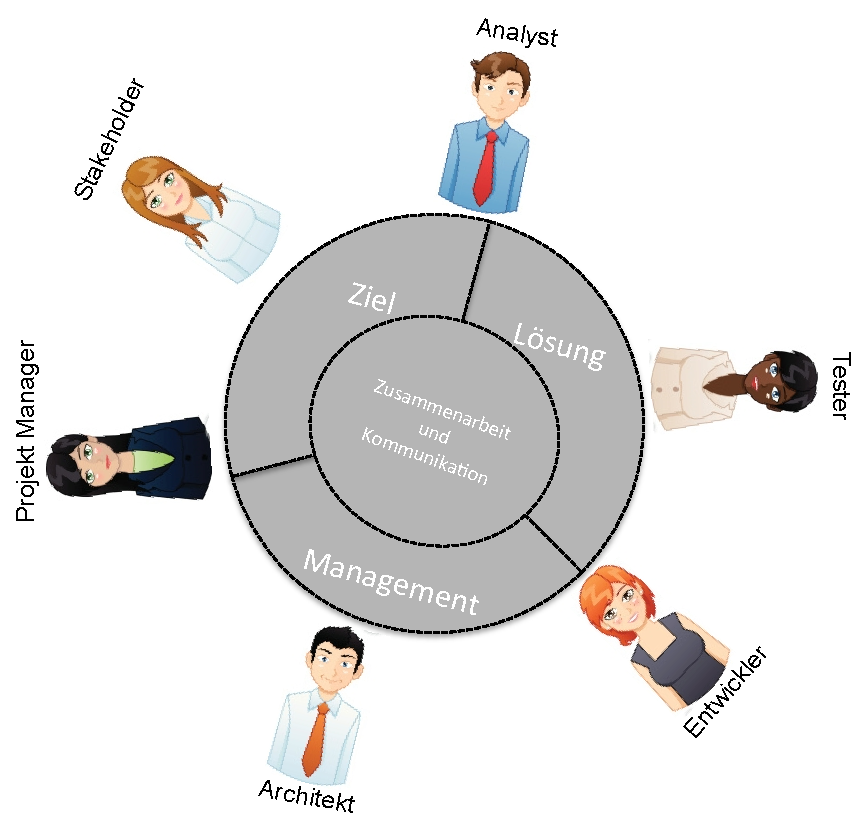
\includegraphics[scale=0.6]{RollenOpenUp} %pdf, jpg, png...
  \caption{Rollen in Open Up nach \cite{openup}}
  \label{fig:RollenOpenUp}
\end{center}
\end{figure}

Eine Task bezeichnet in Open Up die Arbeitseinheit einer Rolle, welche von dieser durchgeführt werden soll. Insgesamt gibt es 18 Tasks, welche von den verschiedenen Rollen entweder als Primär-Darsteller(der Verantwortliche für die Durchführung der Aufgabe) oder als zusätzlicher Darsteller(Unterstützung und Bereitstellung von Informationen, die in der Task- Ausführung verwendet werden) durchgeführt werden. Hierdurch wird der kollaborative Charakter von Open Up gefestigt \cite{eclipseopenup}.

Ein Artefakt ist etwas, das hergestellt, modifiziert oder durch eine Task verwendet wird. Rollen sind 
für die Erstellung und Aktualisierung von Artefakten verantwortlich. Artefakte stellen eine Versionskontrolle während des gesamten Projektlebenszyklus dar. Die 17 Artefakte in OpenUP gelten als die wesentlichen Artefakte, welche ein Projekt verwenden sollte, um produkt- und projektbezogene Informationen zu erfassen. Die Informationen müssen hierbei nicht mit formalen Artefakten festgehalten werden, dies kann auch informell, z.B durch White-Boards oder Meeting-Notizen geschehen. Es können die Open Up Artefakte oder eigene Artefakte verwendet werden \cite{eclipseopenup}.

\subsection{Imperative Modellierung Open Up}

\subsubsection{Develop Solution Increment}

 Bei der Aktivität \textit{Develop Solution Increment} geht es um das Design, die Implementierung, das Testen und die Integration der Lösung für eine Anforderung in einem bestimmten Kontext. Sie tritt genauso viele Male auf, wie es Arbeitsaufgaben gibt, die in einer Iteration entwickelt werden müssen.
 Handelt es sich um eine typische Veränderung wird zunächst eine Lösung designt und anschließend ein Entwickeltest implementiert. Bei einer trivialen Änderung an der bestehenden Implementierung kann diese auch direkt in der bestehenden Architektur vorgenommen werden. \newline
 Sobald die Fragen der technischen Umsetzung geklärt sind, werden Entwicklertests implementiert, um die Implementierung zu verifizieren. Anschließend werden diese Entwicklertests ausgeführt.\newline
 Falls bei der Ausführung der Tests Fehler ersichtlich werden, muss eine Lösung für diesen Fehler implementiert werden und die Entwicklertests müssen erneut ausgeführt werden. Dies wird solange wiederholt, bis alle Tests bestanden sind.\newline
 Auch wenn alle Tests bestanden werden, sollte der Entwurf an dieser Stelle nochmals überdacht werden. Falls hier beschlossen wird, dass der Code überarbeitet werden muss, muss im Prozess zurückgegangen werden und erneut eine Lösung designt werden, da eine Änderung des Codes die Implementation und die Entwicklertests beeinflussen könnte.\newline
 Da es am Besten ist die Implementierungsteile so klein wie möglich zu halten, sollte zunächst eine kleine Design-Lösung für einen Teil der Arbeitsaufgabe entwickelt werden. Anschließend sollte dies für weitere kleine Teile solange wiederholt werden, bis die gesamte Arbeitsaufgabe implementiert ist. \newline
 
 
\begin{figure}[htp]
\begin{center}
  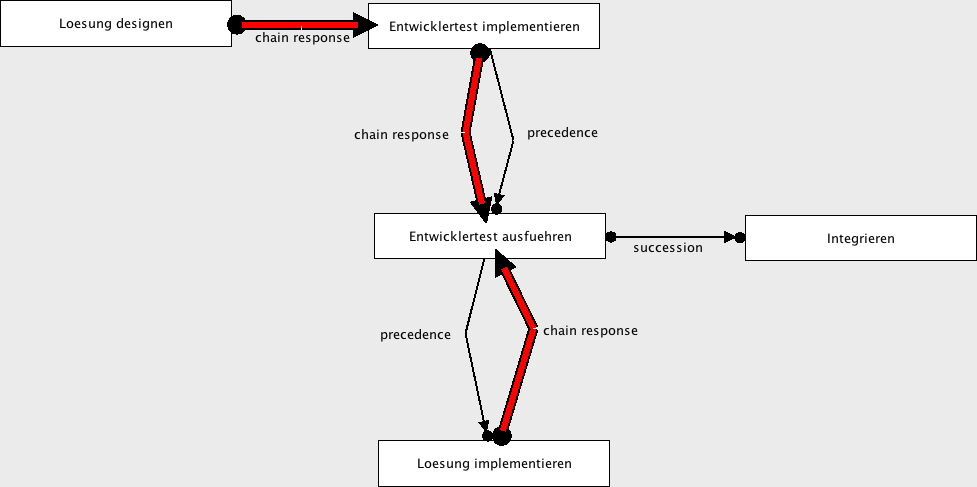
\includegraphics[width=\linewidth]{DevelopSolution} %pdf, jpg, png...
  \caption{Develop Solution Increment imperativ}
  \label{fig:Develop}
\end{center}
\end{figure}

\subsubsection{Plan and manage iteration- Inception}

Die Aktivität \textit{Plan and manage iteration} wird während des gesamten Projektlebenszyklus ausgeführt. Ihr Ziel ist es, Risiken und Probleme früh genug zu identifizieren, damit diese entschärft werden können, um die Ziele für die Iteration festzulegen und das Team dabei zu unterstützen, diese zu erreichen.\newline
Die iteration wird durch den Projektmanager und das Team gestartet. Hier findet die Priorisierung der Arbeit für eine gegebene Iteration statt. Der Projektmanager, die Stakeholder und die Teammitglieder einigen sich darauf, was während der Iteration zu entwickeln ist.\newline
Die Teammitglieder melden sich für die Arbeitsaufgaben, die während der Iteration entwickelt werden müssen. Anschließend teilt sich jedes Teammitglied seine Arbeitsaufgaben selbstständig in Arbeitseinheiten ein und schätzt den Aufwand hierfür ab.\newline
Während der Iteration trifft sich das Team regelmäßig, um den aktuellen Stand der Arbeit und eventuelle Probleme zu besprechen.


\begin{figure}[htp]
\begin{center}
  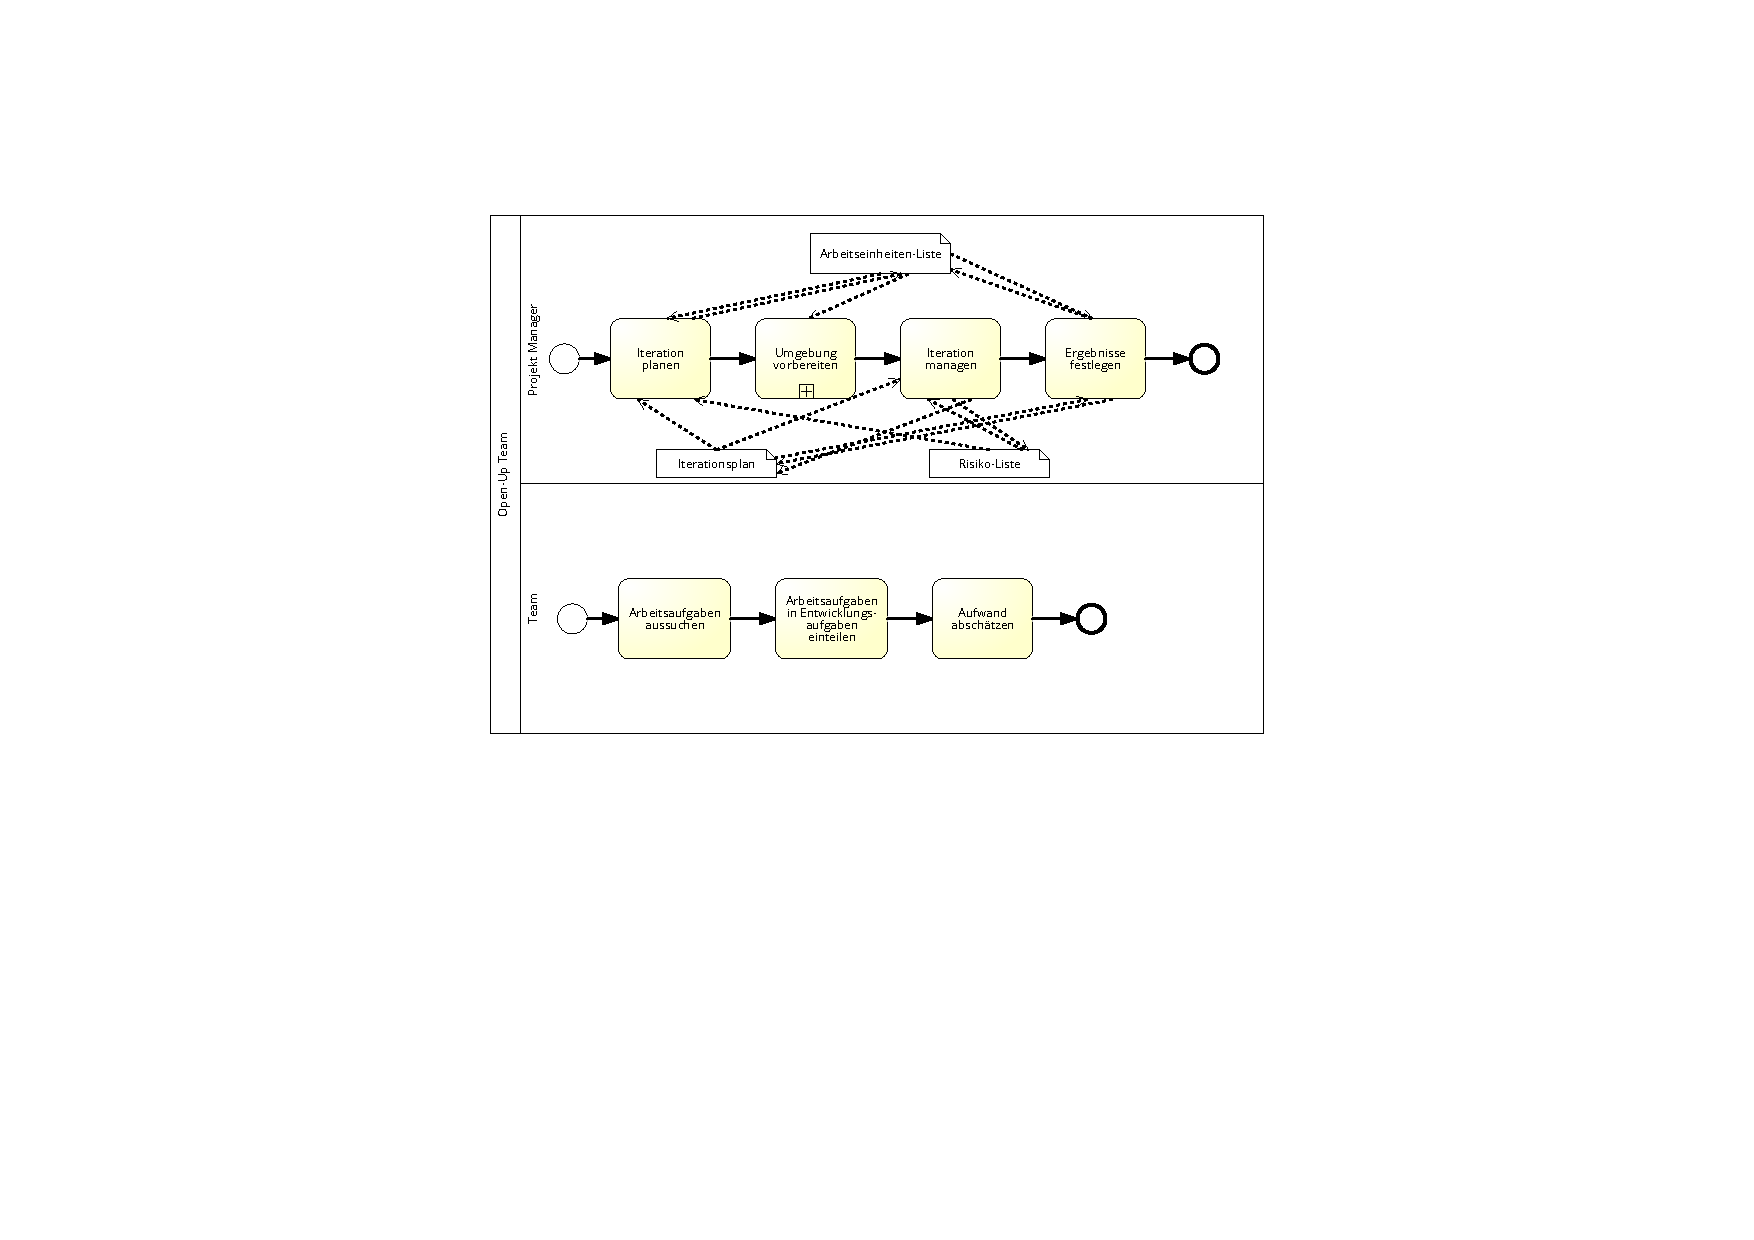
\includegraphics[width=\linewidth]{PlanAndManageIterationInception-2} %pdf, jpg, png...
  \caption{Plan and manage iteration imperativ -Inception}
  \label{fig:PlanAndManageIterationInception-2}
\end{center}
\end{figure}

\begin{figure}[htp]
\begin{center}
  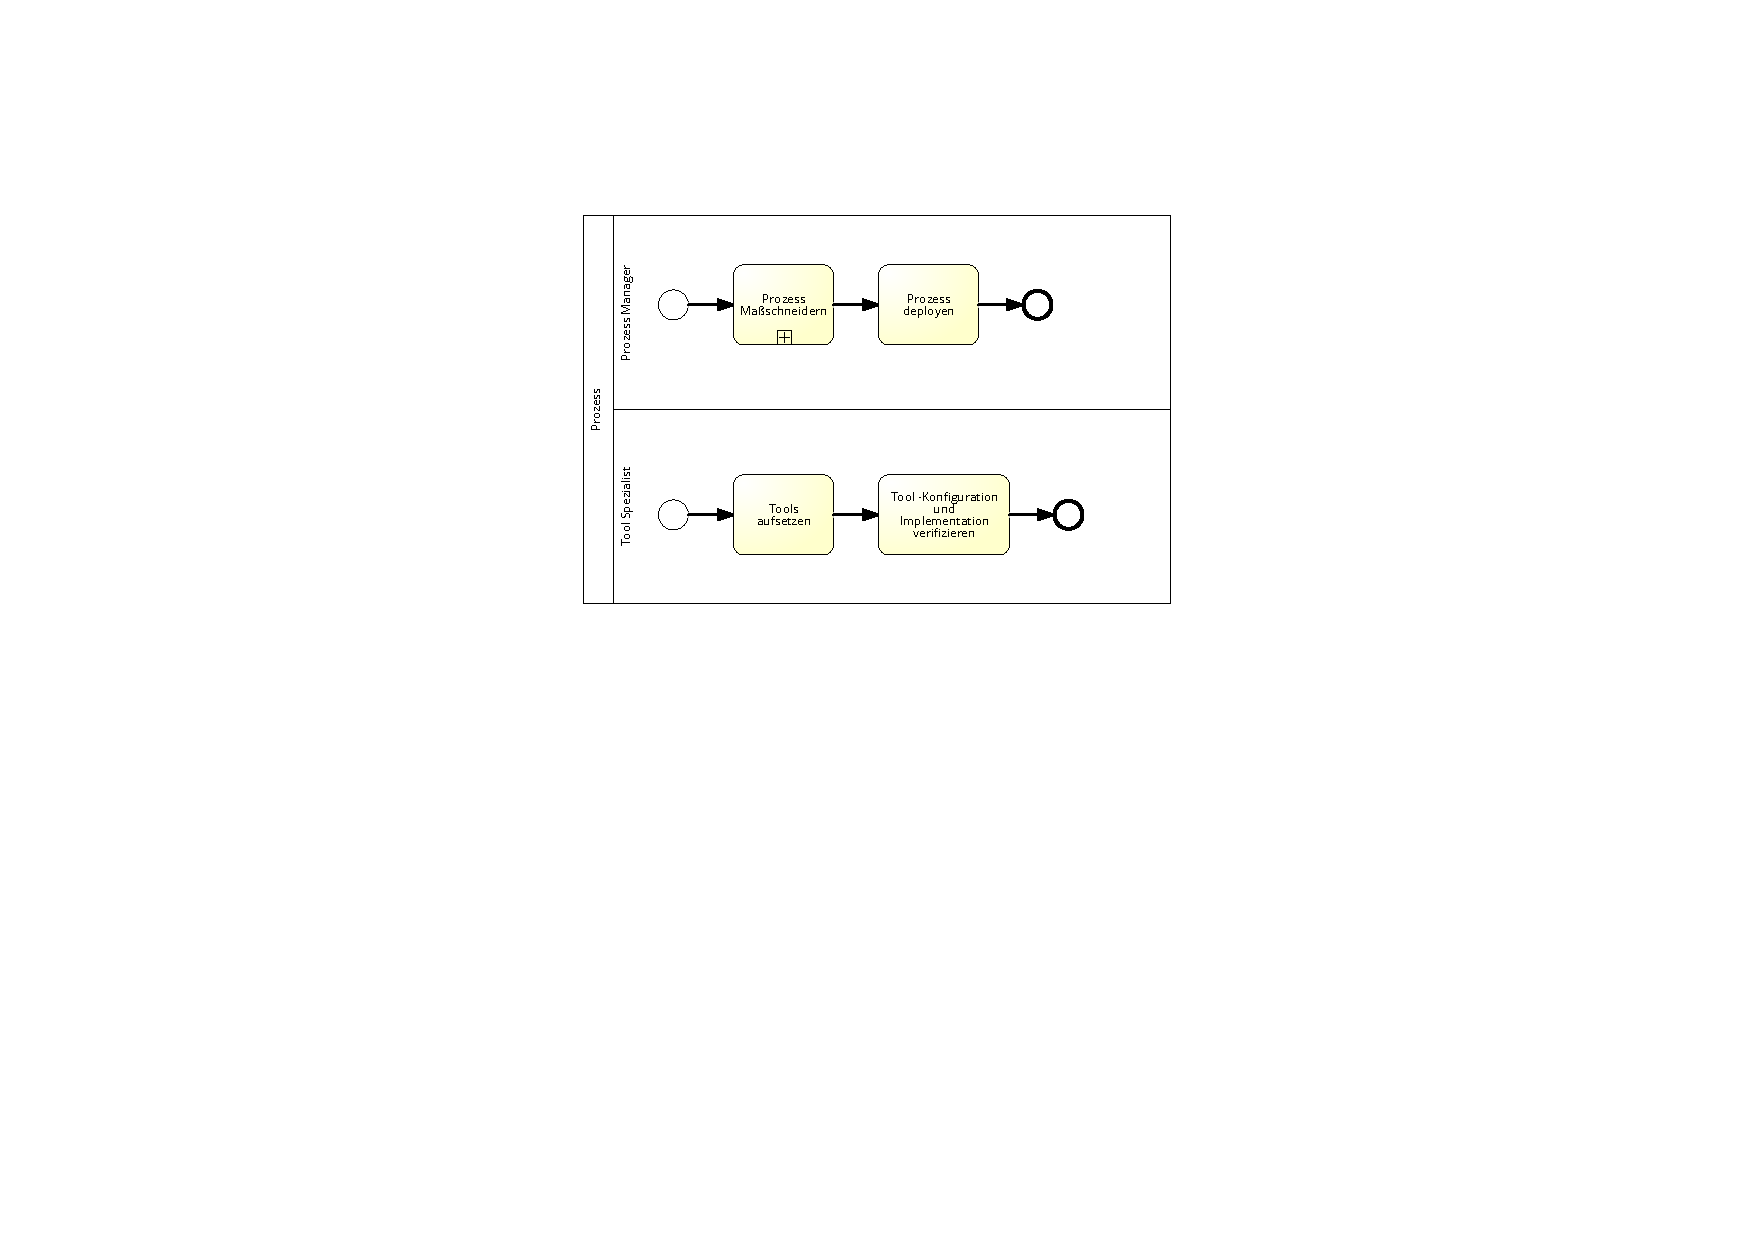
\includegraphics[width=\linewidth]{PlanAndManageIterationInception-2Unter} %pdf, jpg, png...
  \caption{Plan and manage iteration imperativ -Inception Unterprozess Umgebung vorbereiten} 
  \label{fig:PlanAndManageIterationInception-2}
\end{center}
\end{figure}


\begin{figure}[htp]
\begin{center}
  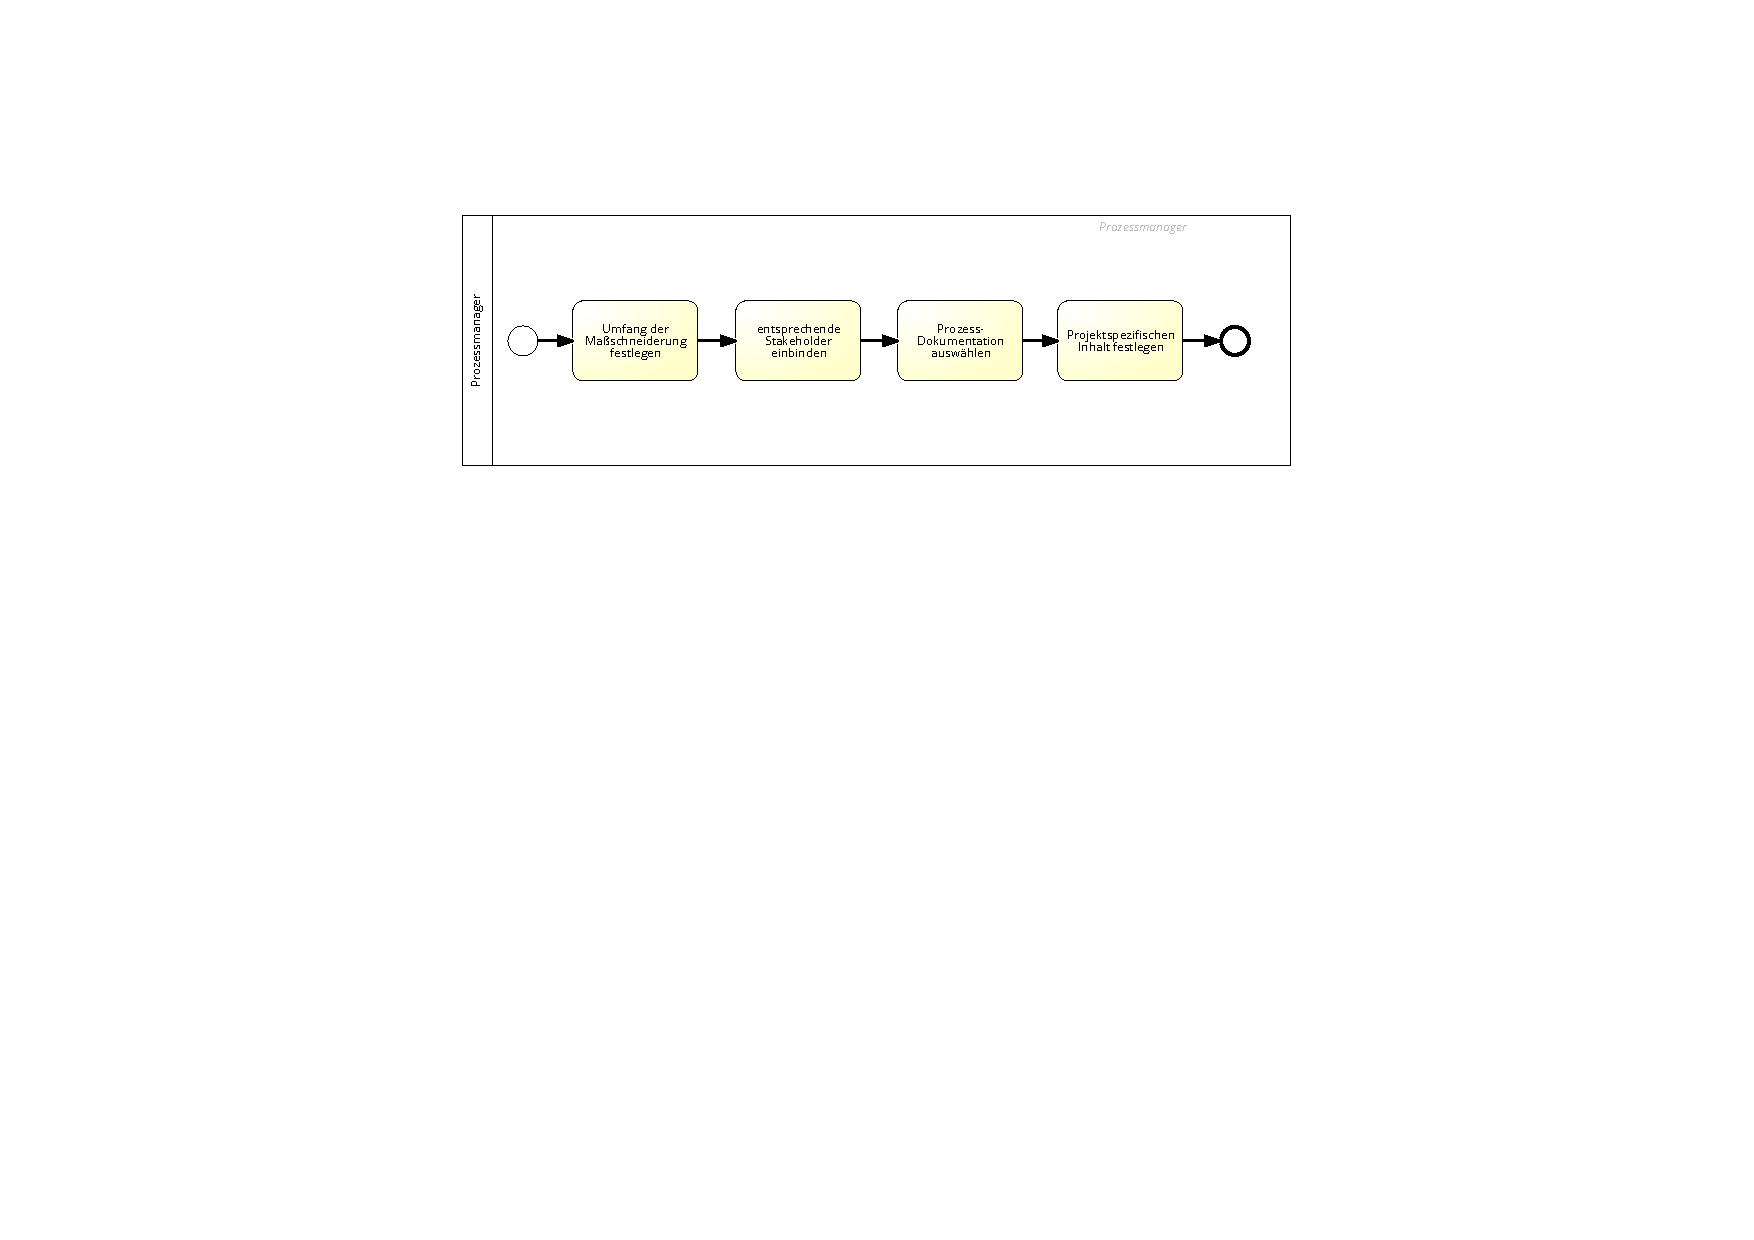
\includegraphics[width=\linewidth]{PlanAndManageIterationInception-2UnterUnter} %pdf, jpg, png...
  \caption{Plan and manage iteration imperativ-Inception Unterprozess Prozess maßschneidern}
  \label{fig:PlanAndManageIterationInception-2UnterUnter}
\end{center}
\end{figure}

\subsubsection{Deploy Release-Transition}


Das Ergebnis dieser Aktivität ist die Release eines Sets von integrierten Komponenten in die Integrationsumgebung. 
\begin{figure}[htp]
\begin{center}
  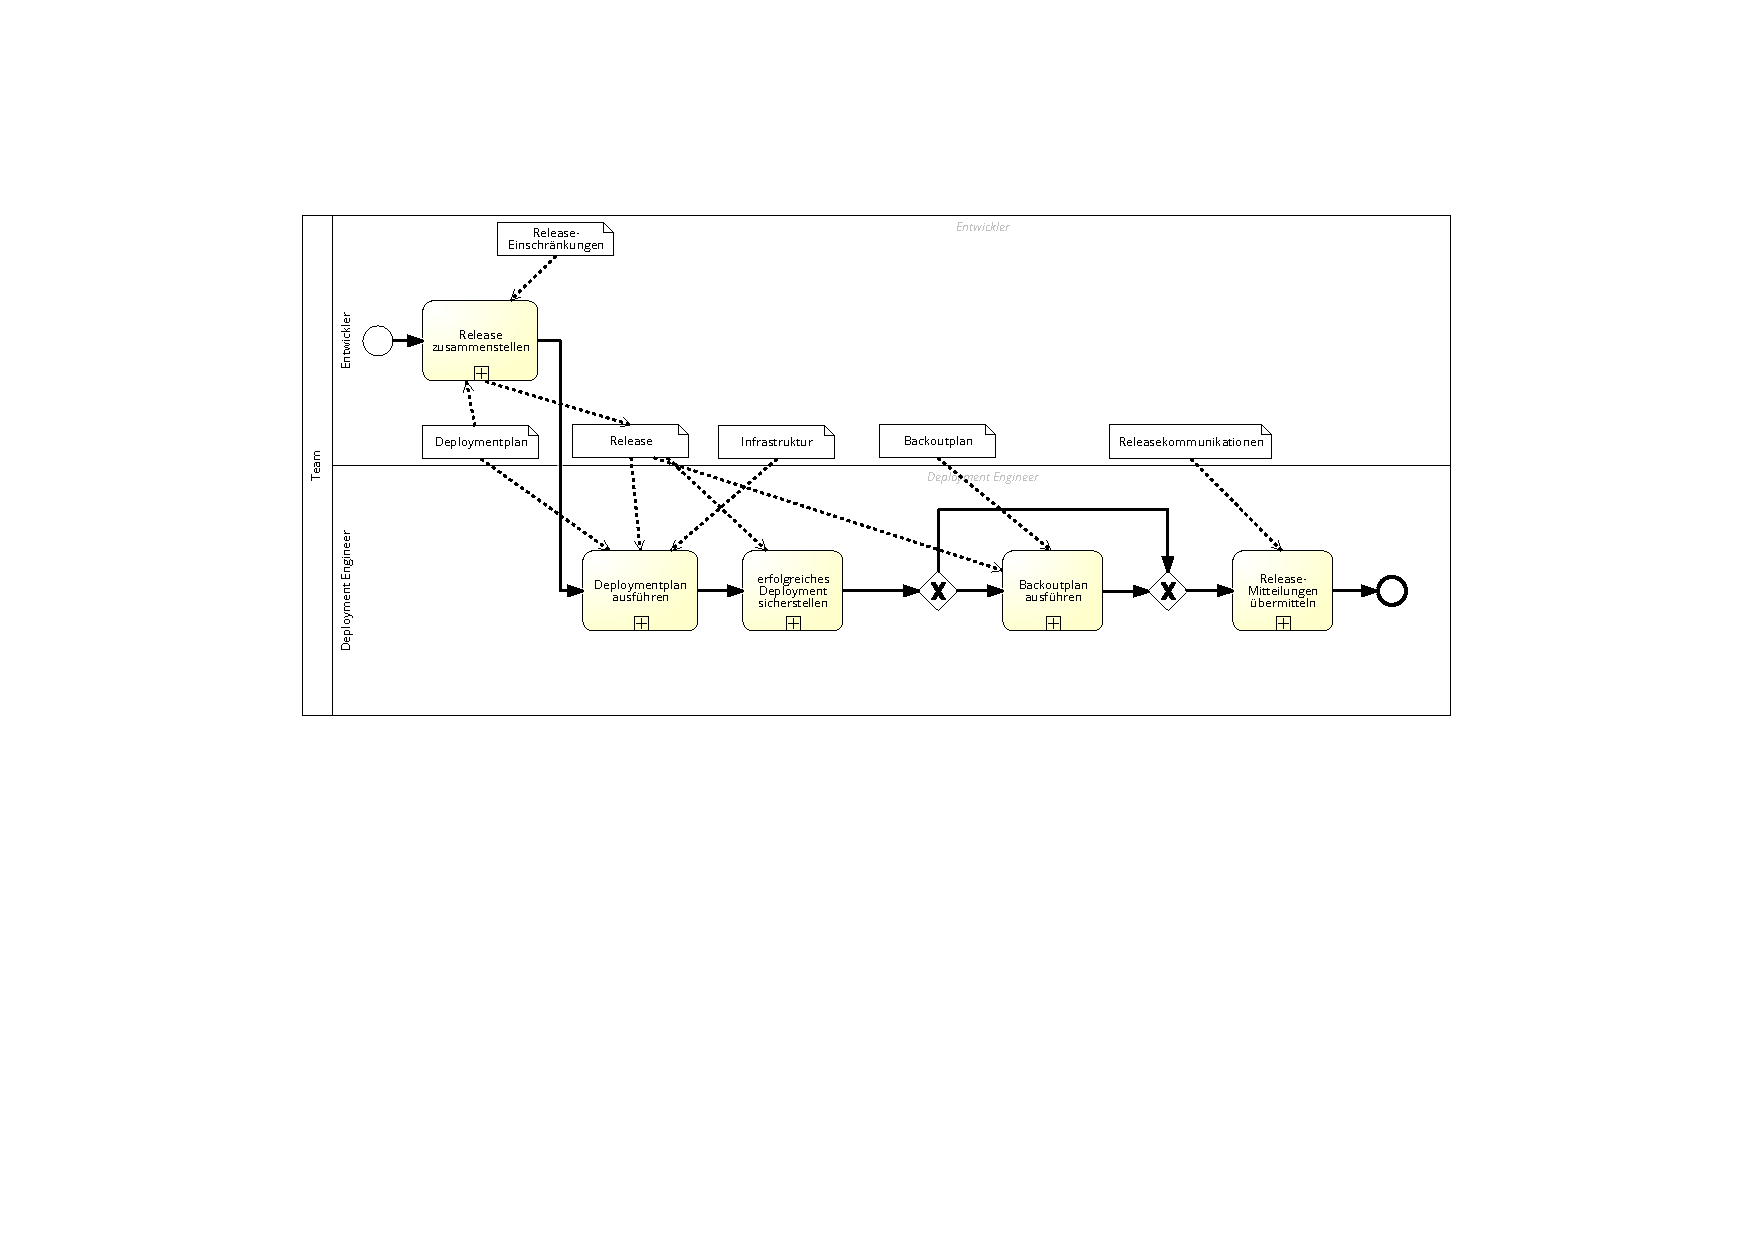
\includegraphics[width=\linewidth]{DeployReleaseTransition} %pdf, jpg, png...
  \caption{Deploy Release-Transition}
  \label{fig:DeployRelease}
\end{center}
\end{figure}

\begin{figure}[htp]
\begin{center}
  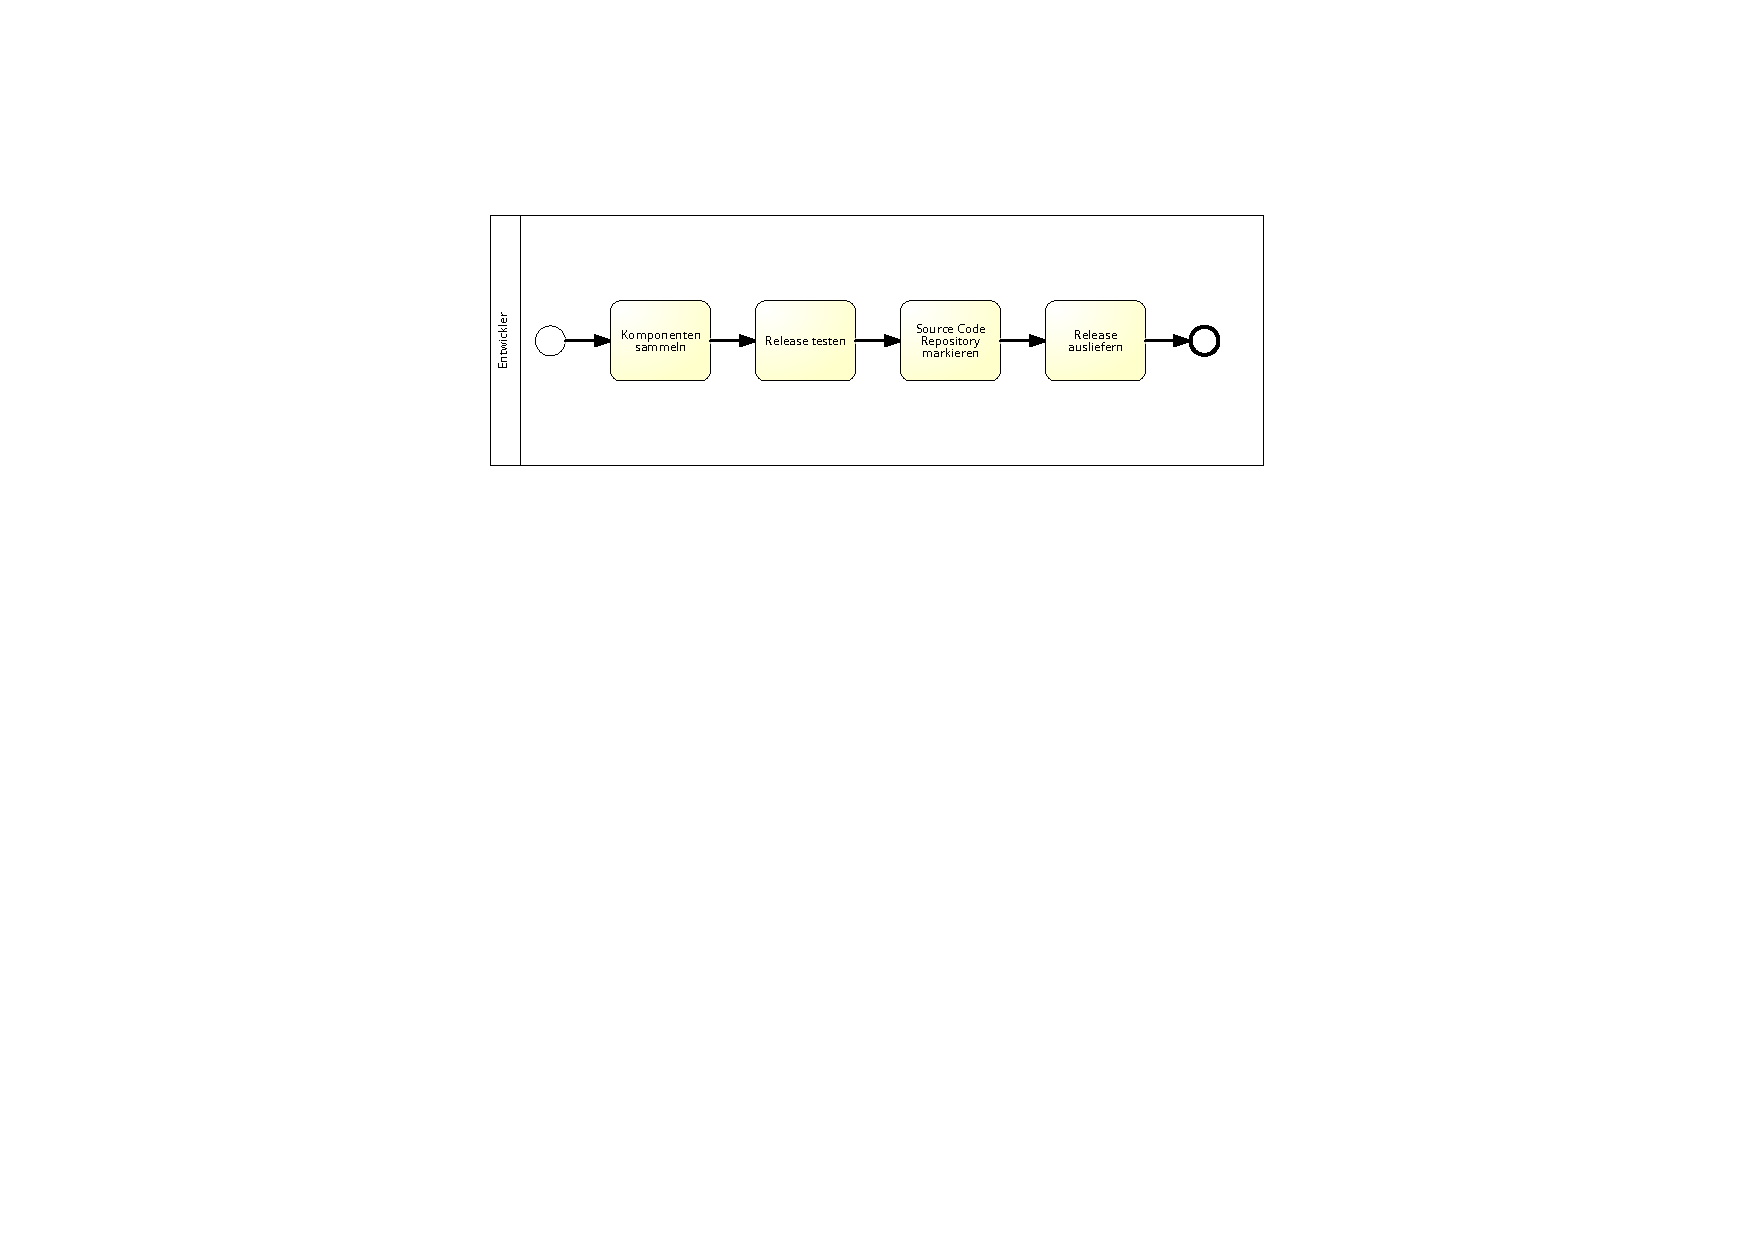
\includegraphics[width=\linewidth]{Releasezusammenstellen} %pdf, jpg, png...
  \caption{Deploy Release-Transition Unterprozess Release zusammen stellen}
  \label{fig:Releasezusammenstellen}
\end{center}
\end{figure}

\begin{figure}[htp]
\begin{center}
  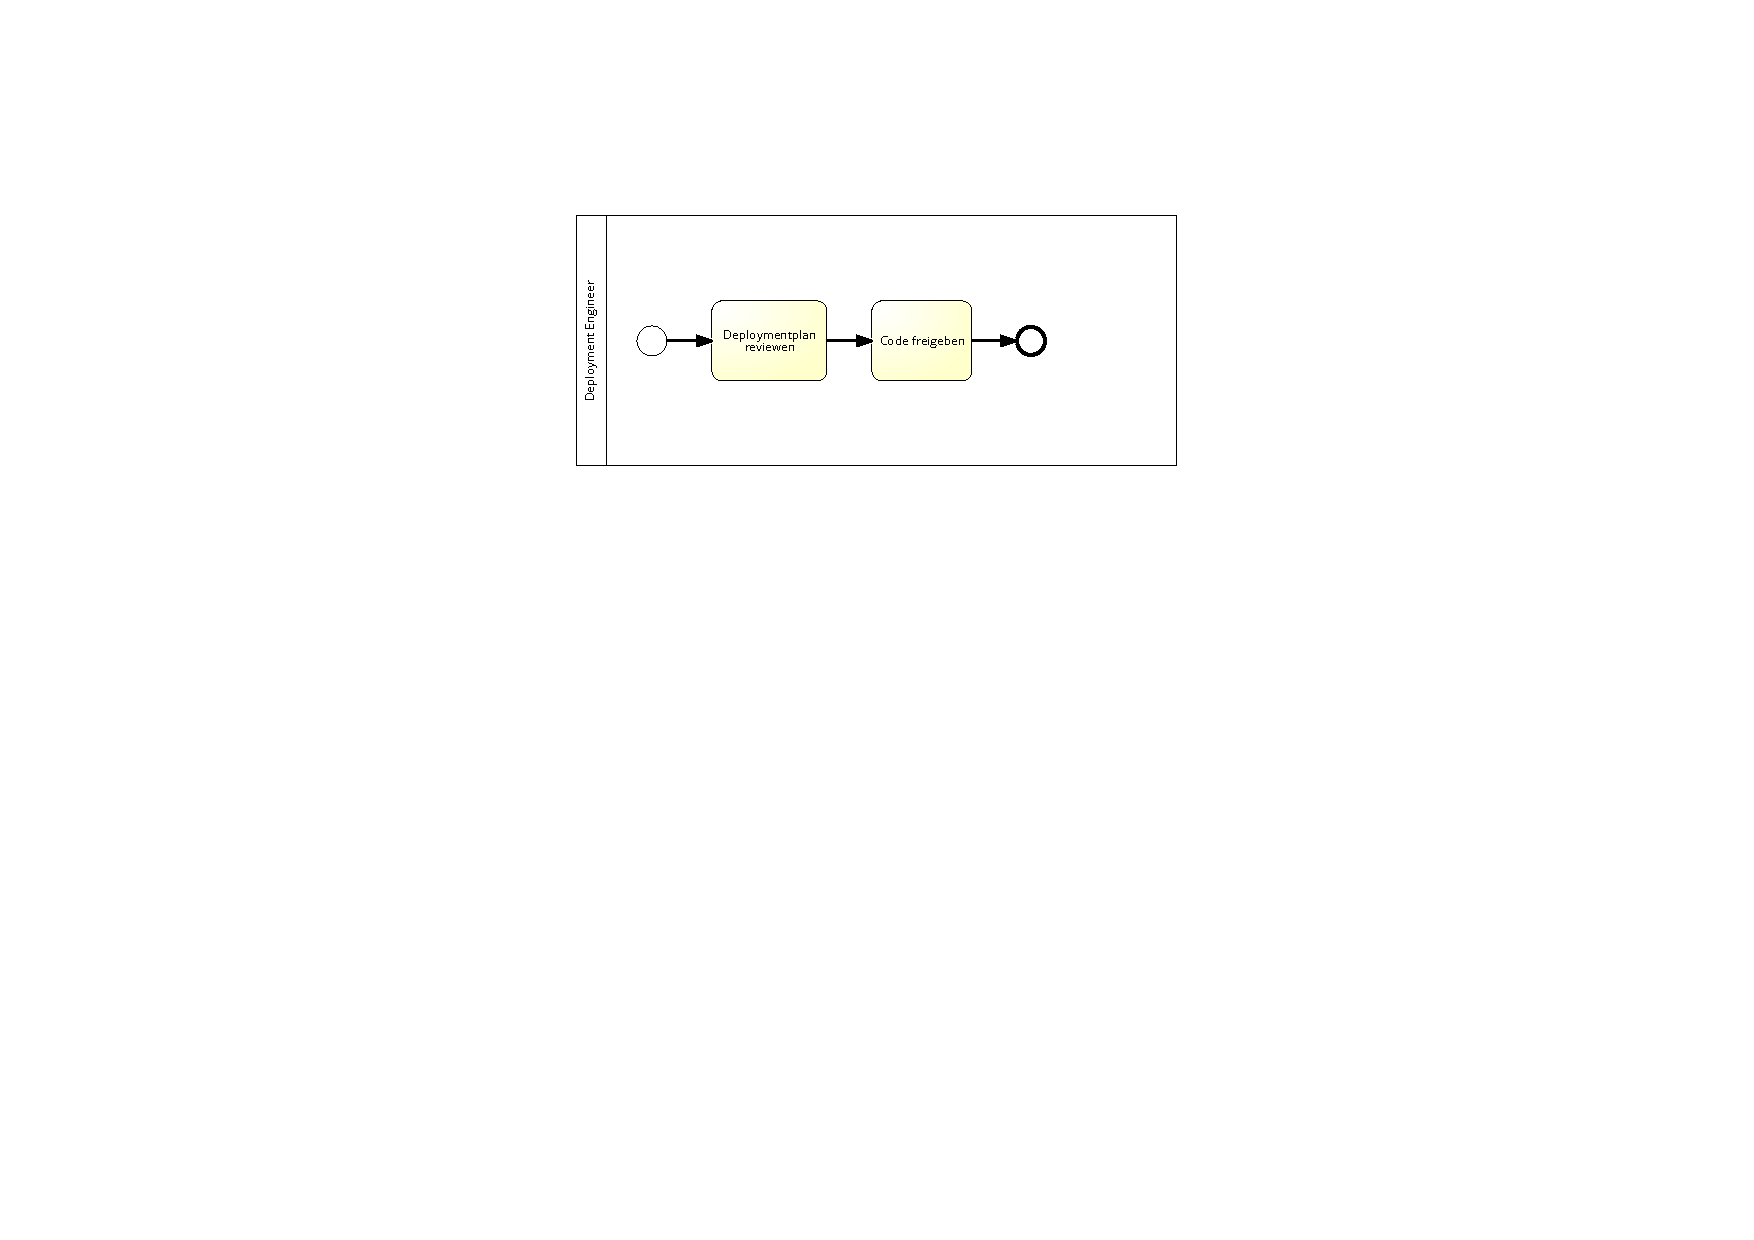
\includegraphics[width=\linewidth]{Deploymentplanausfuhren} %pdf, jpg, png...
  \caption{Deploy Release-Transition Unterprozess Deploymentplan ausführen}
  \label{fig:Deploymentplanausfuhren}
\end{center}
\end{figure}

\begin{figure}[htp]
\begin{center}
  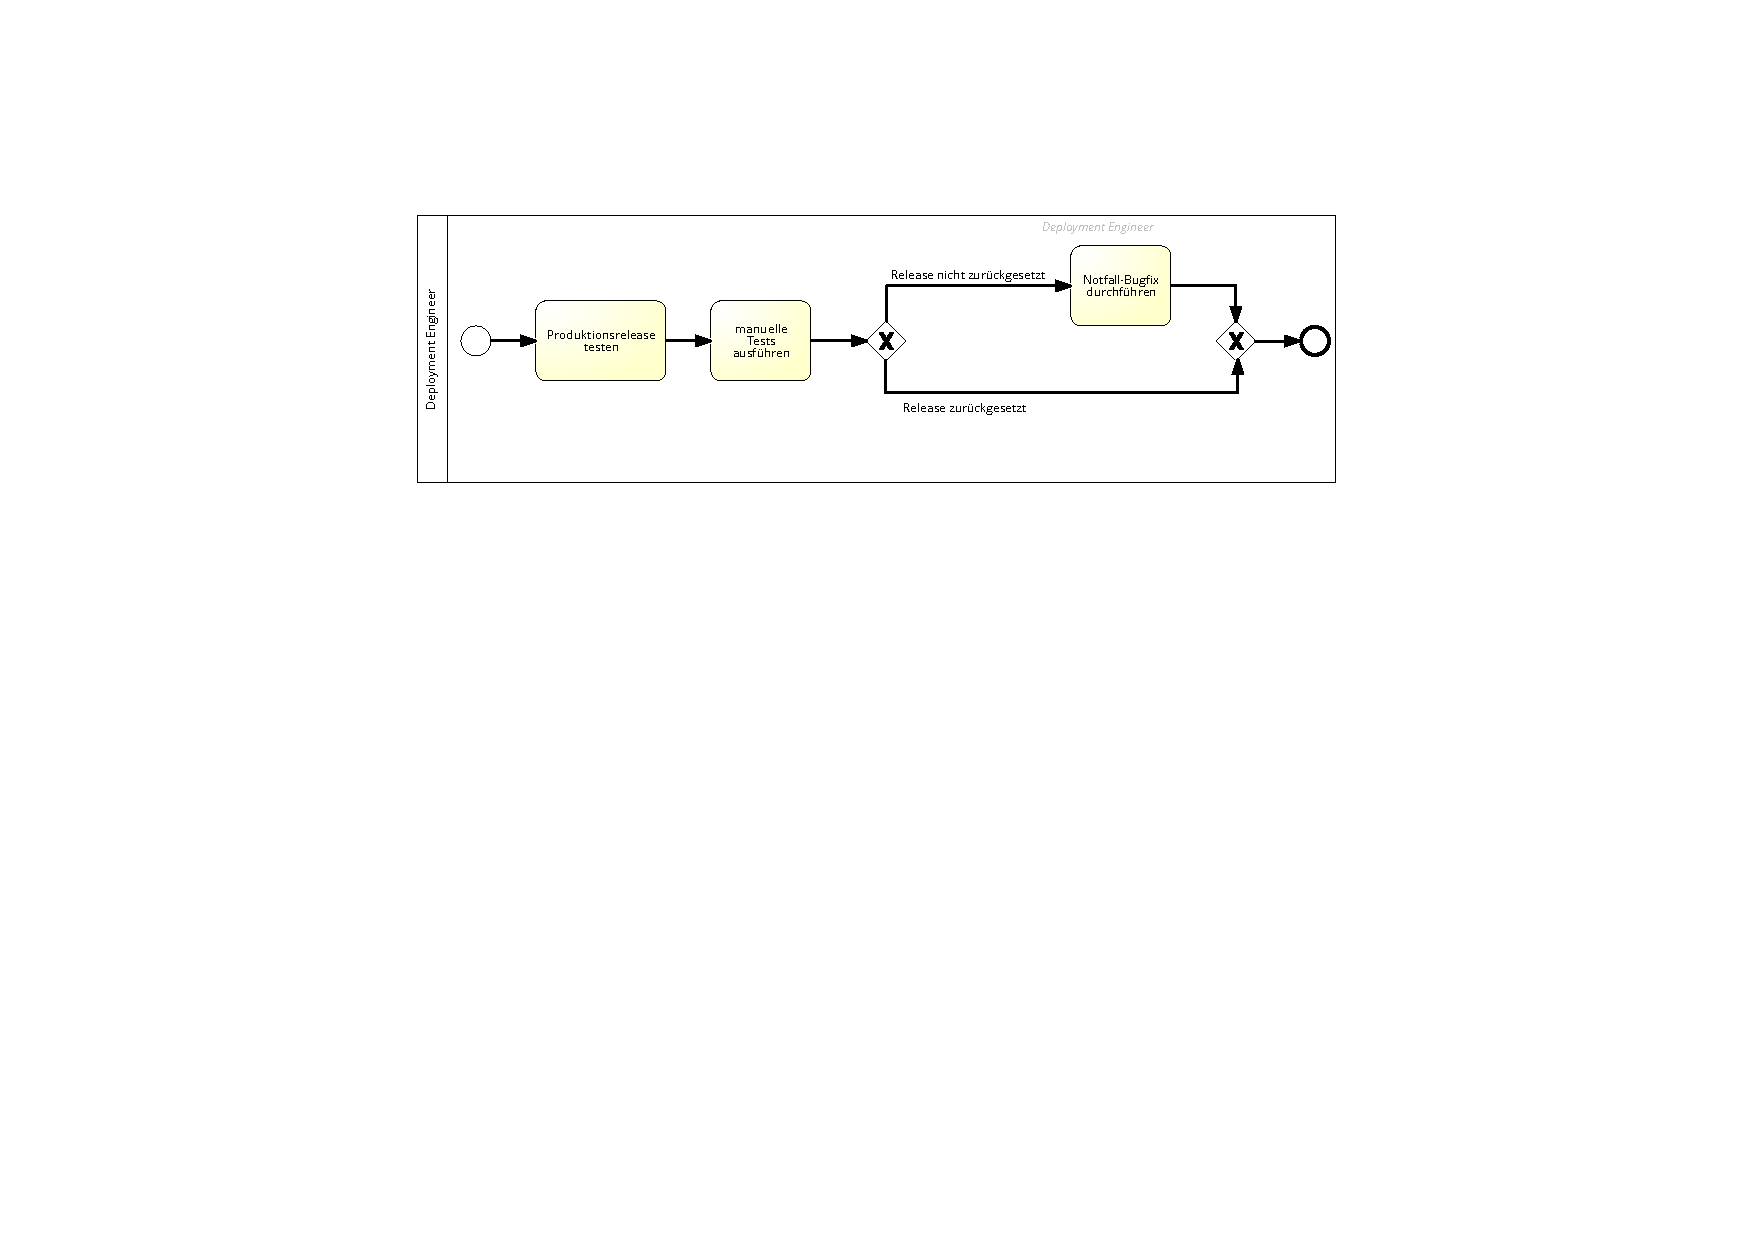
\includegraphics[width=\linewidth]{erfolgreichesDeploymentsicherstellen} %pdf, jpg, png...
  \caption{Deploy Release-Transition Unterprozess Erfolgreiches Deployment sicherstellen}
  \label{fig:erfolgreichesDeploymentsicherstellen}
\end{center}
\end{figure}

\begin{figure}[htp]
\begin{center}
  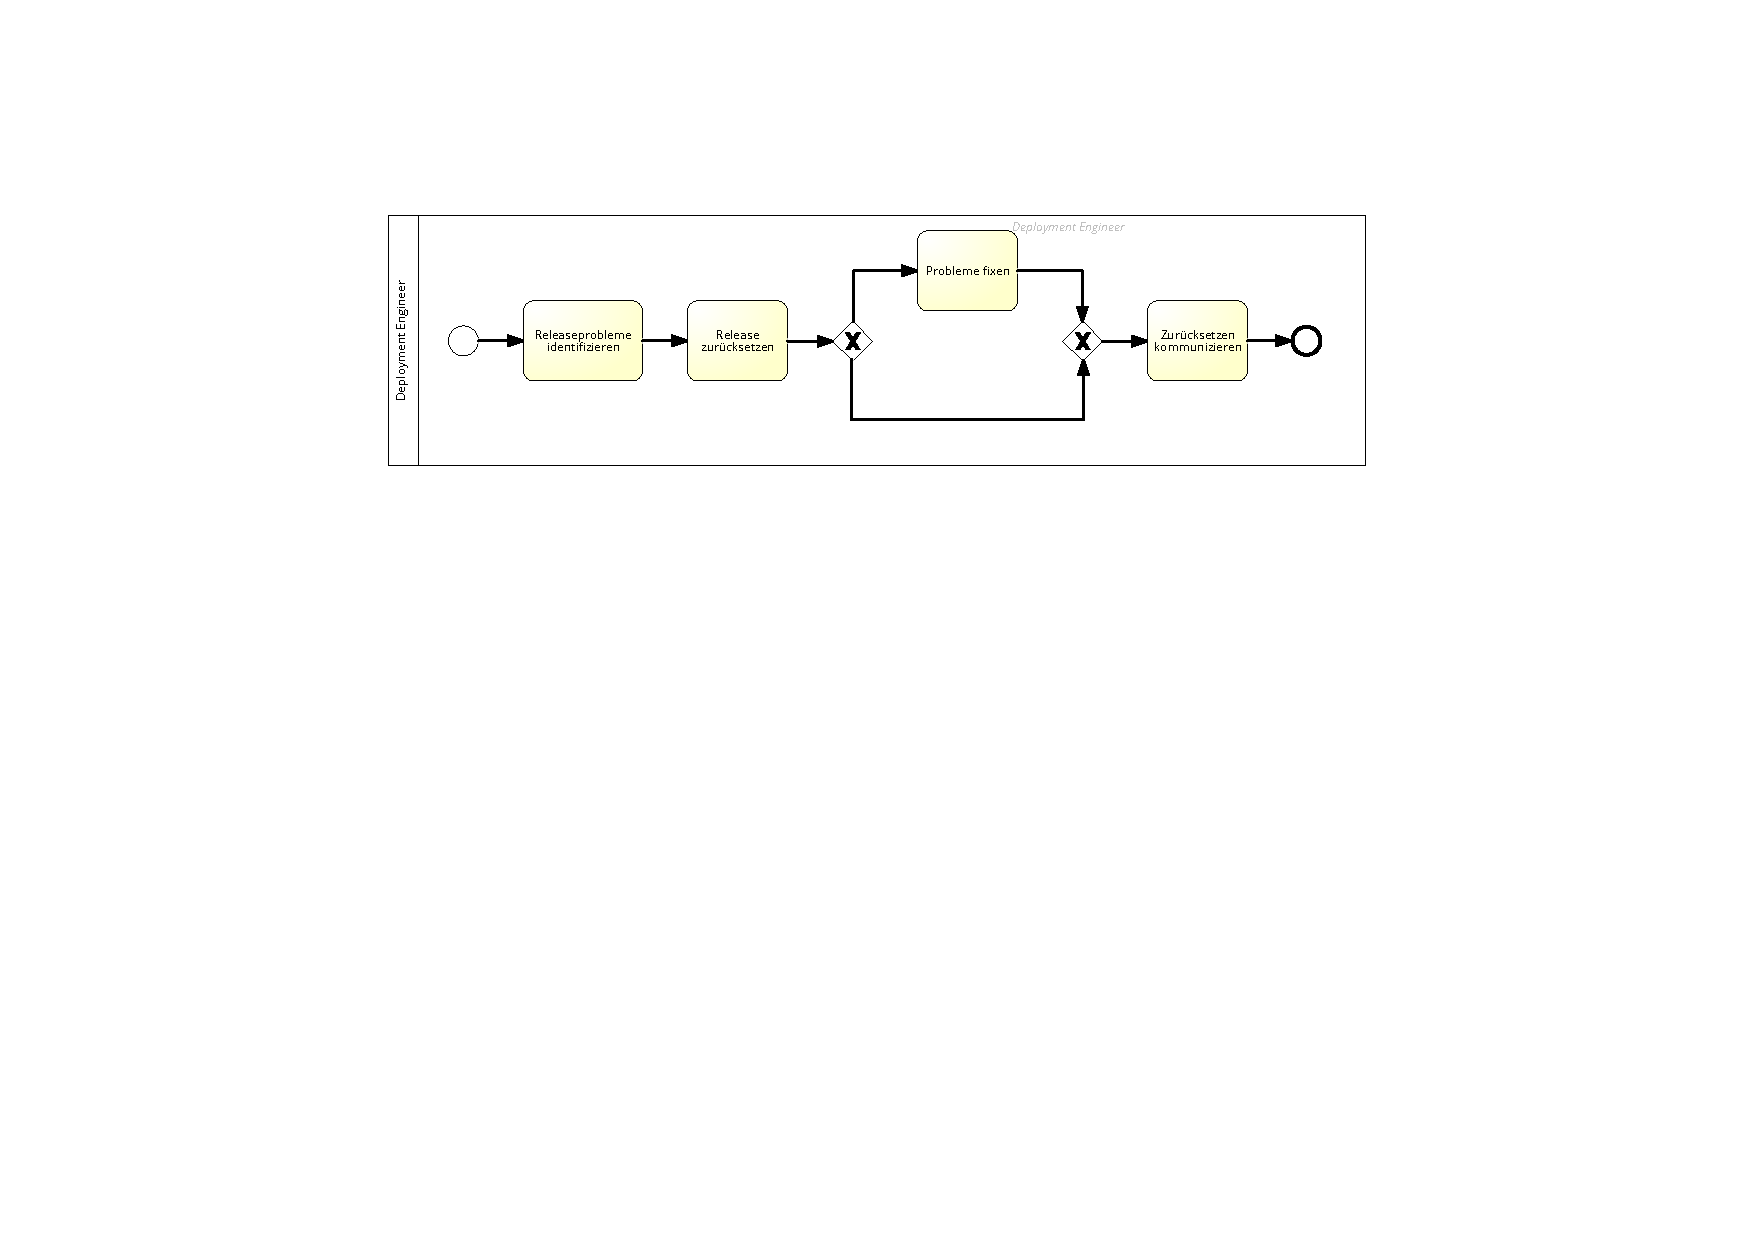
\includegraphics[width=\linewidth]{Backoutplanausfuhren} %pdf, jpg, png...
  \caption{Deploy Release-Transition Unterprozess Backoutplan ausführen}
  \label{fig:Backoutplanausfuhren}
\end{center}
\end{figure}


\begin{figure}[htp]
\begin{center}
  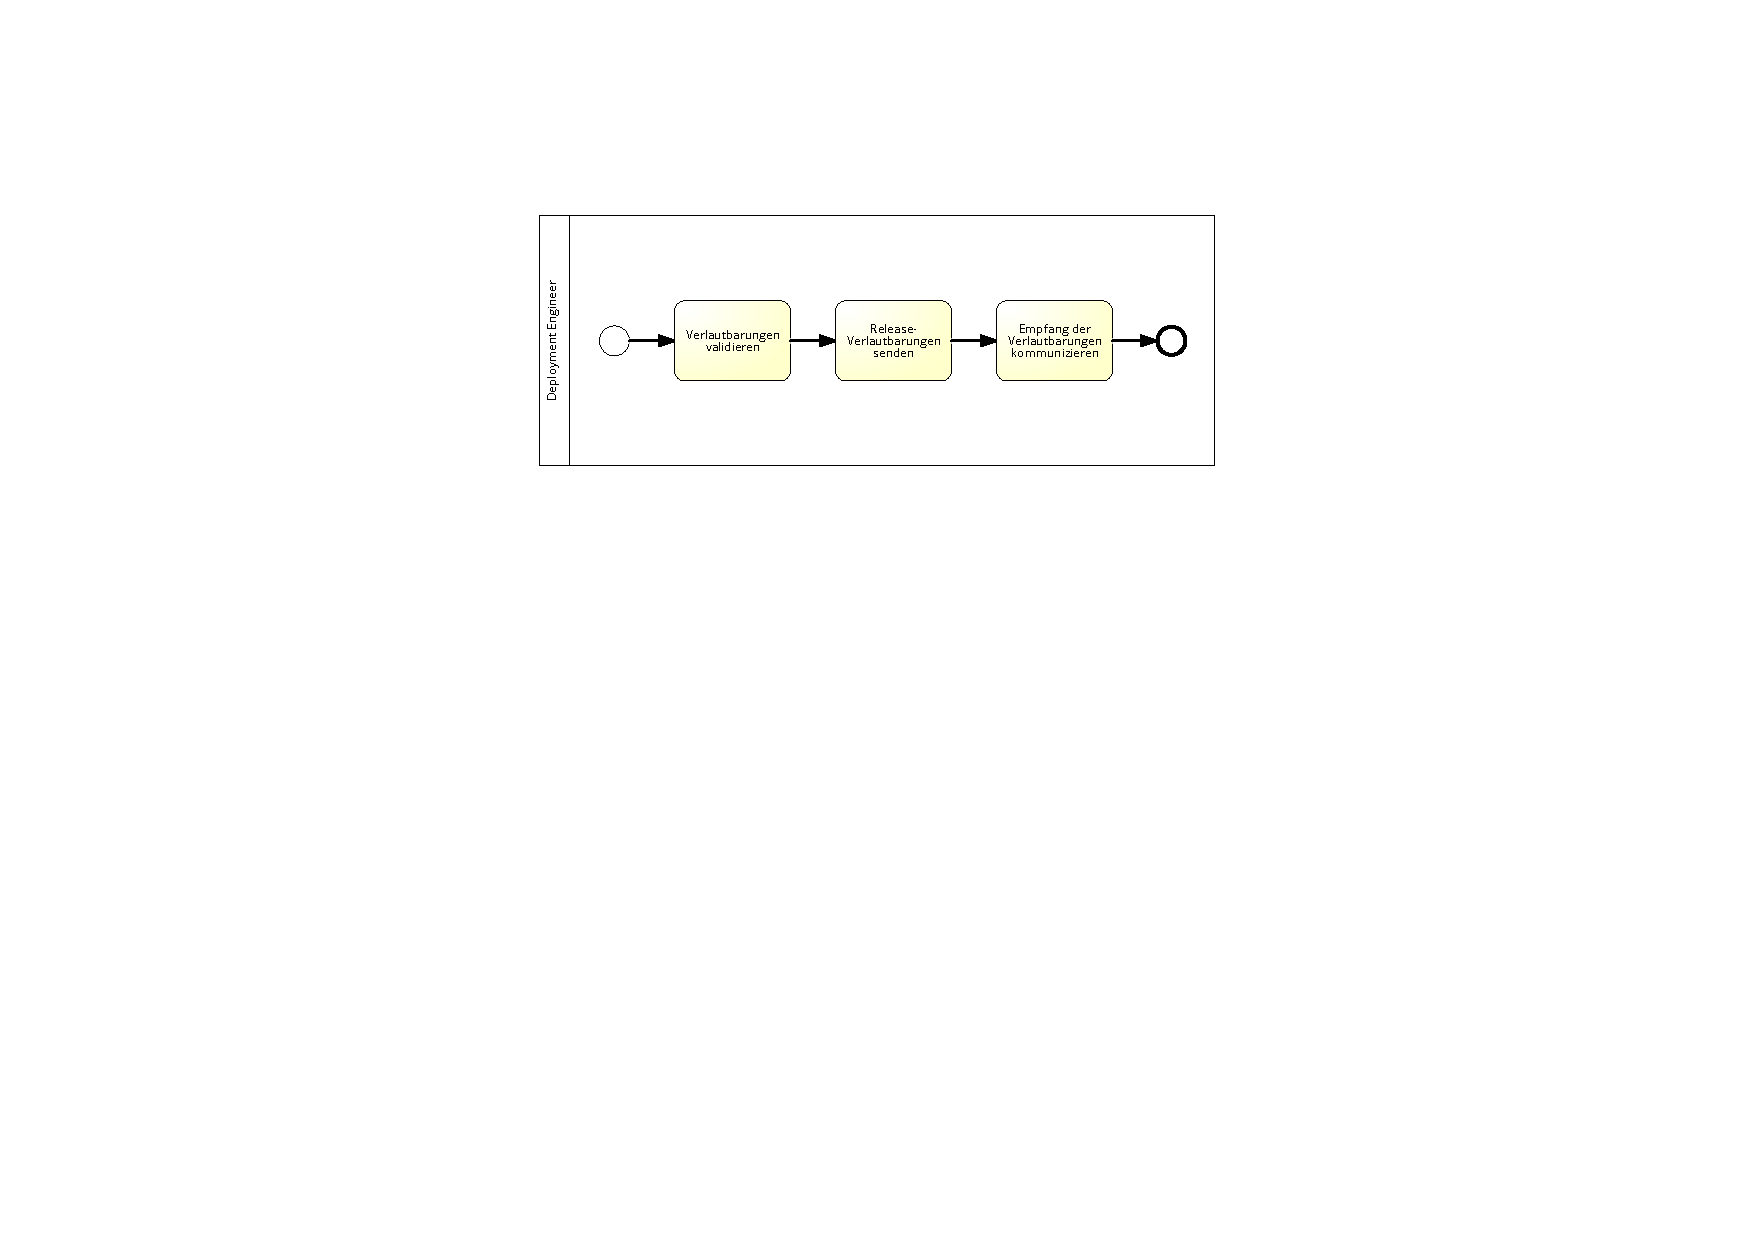
\includegraphics[width=\linewidth]{ReleaseMitteilungenubermitteln} %pdf, jpg, png...
  \caption{Deploy Release-Transition Unterprozess Release Mitteilungen übermitteln}
  \label{fig:Backoutplanausfuhren}
\end{center}
\end{figure}

\subsubsection{Develop Product Documentation-Construction}

\begin{figure}[htp]
\begin{center}
  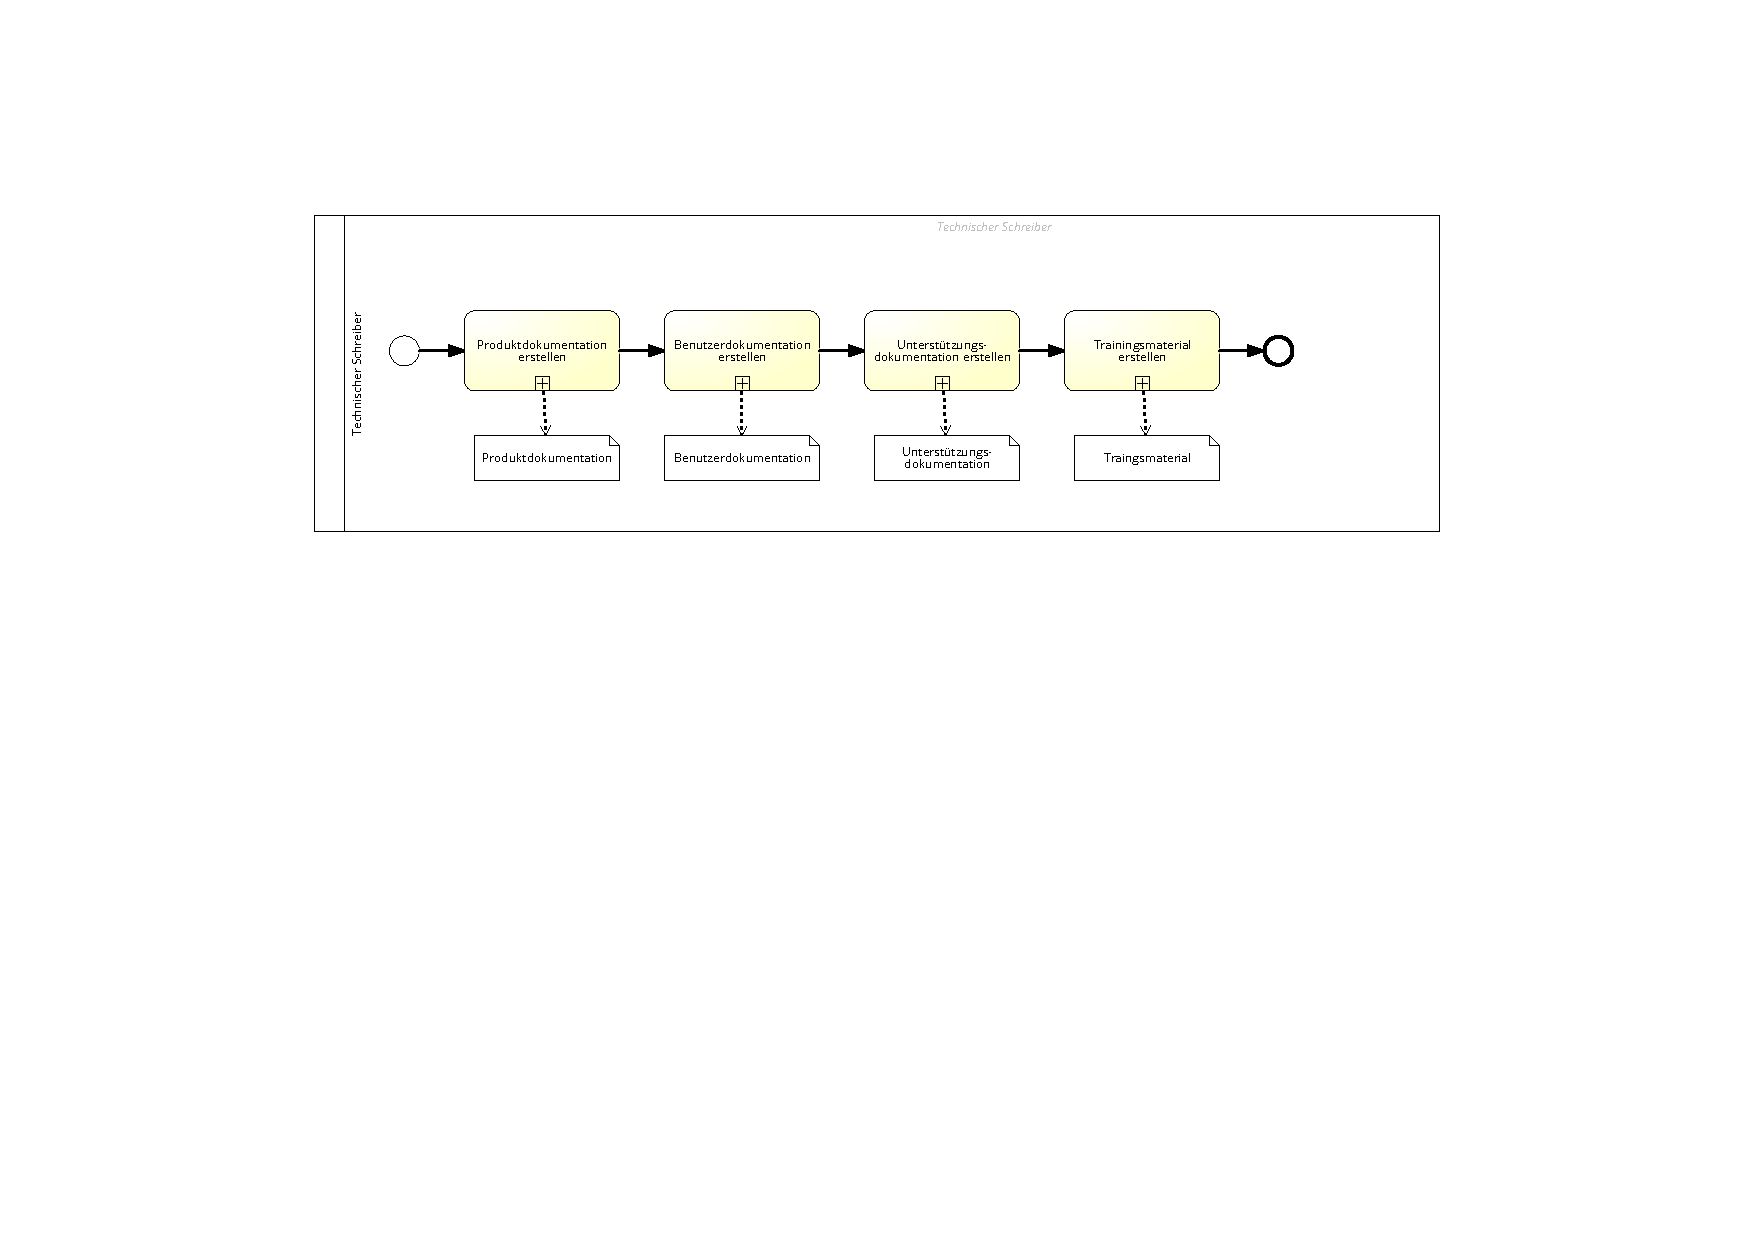
\includegraphics[width=\linewidth]{DevelopProductDocumentation} %pdf, jpg, png...
  \caption{Develop Product Documentation-Construction}
  \label{fig:DevelopProductDocumentation}
\end{center}
\end{figure}

\begin{figure}[htp]
\begin{center}
  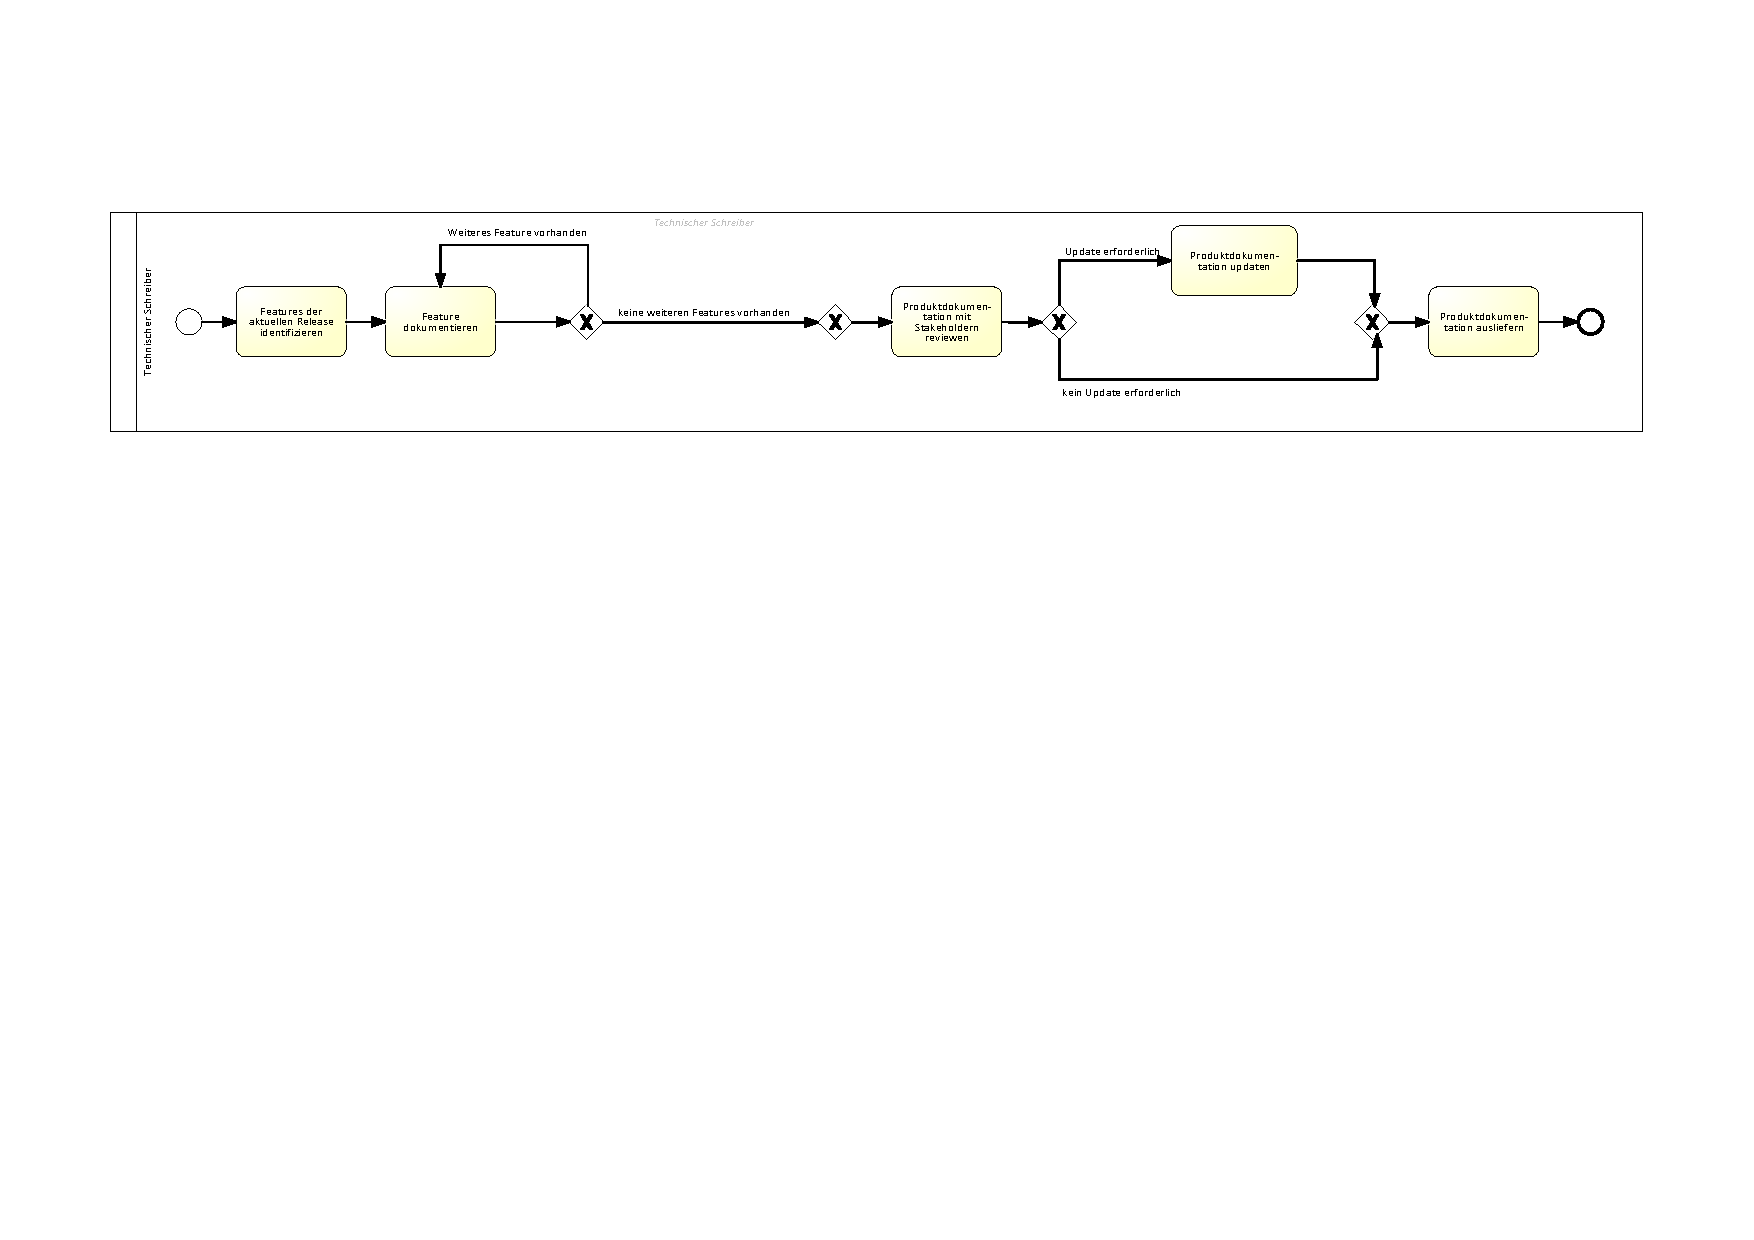
\includegraphics[width=\linewidth]{ProduktdokumentationErstellen} %pdf, jpg, png...
  \caption{Develop Product Documentation-Construction Unterprozess Produktdokumentation erstellen}
  \label{fig:ProduktdokumentationErstellen}
\end{center}
\end{figure}

\begin{figure}[htp]
\begin{center}
  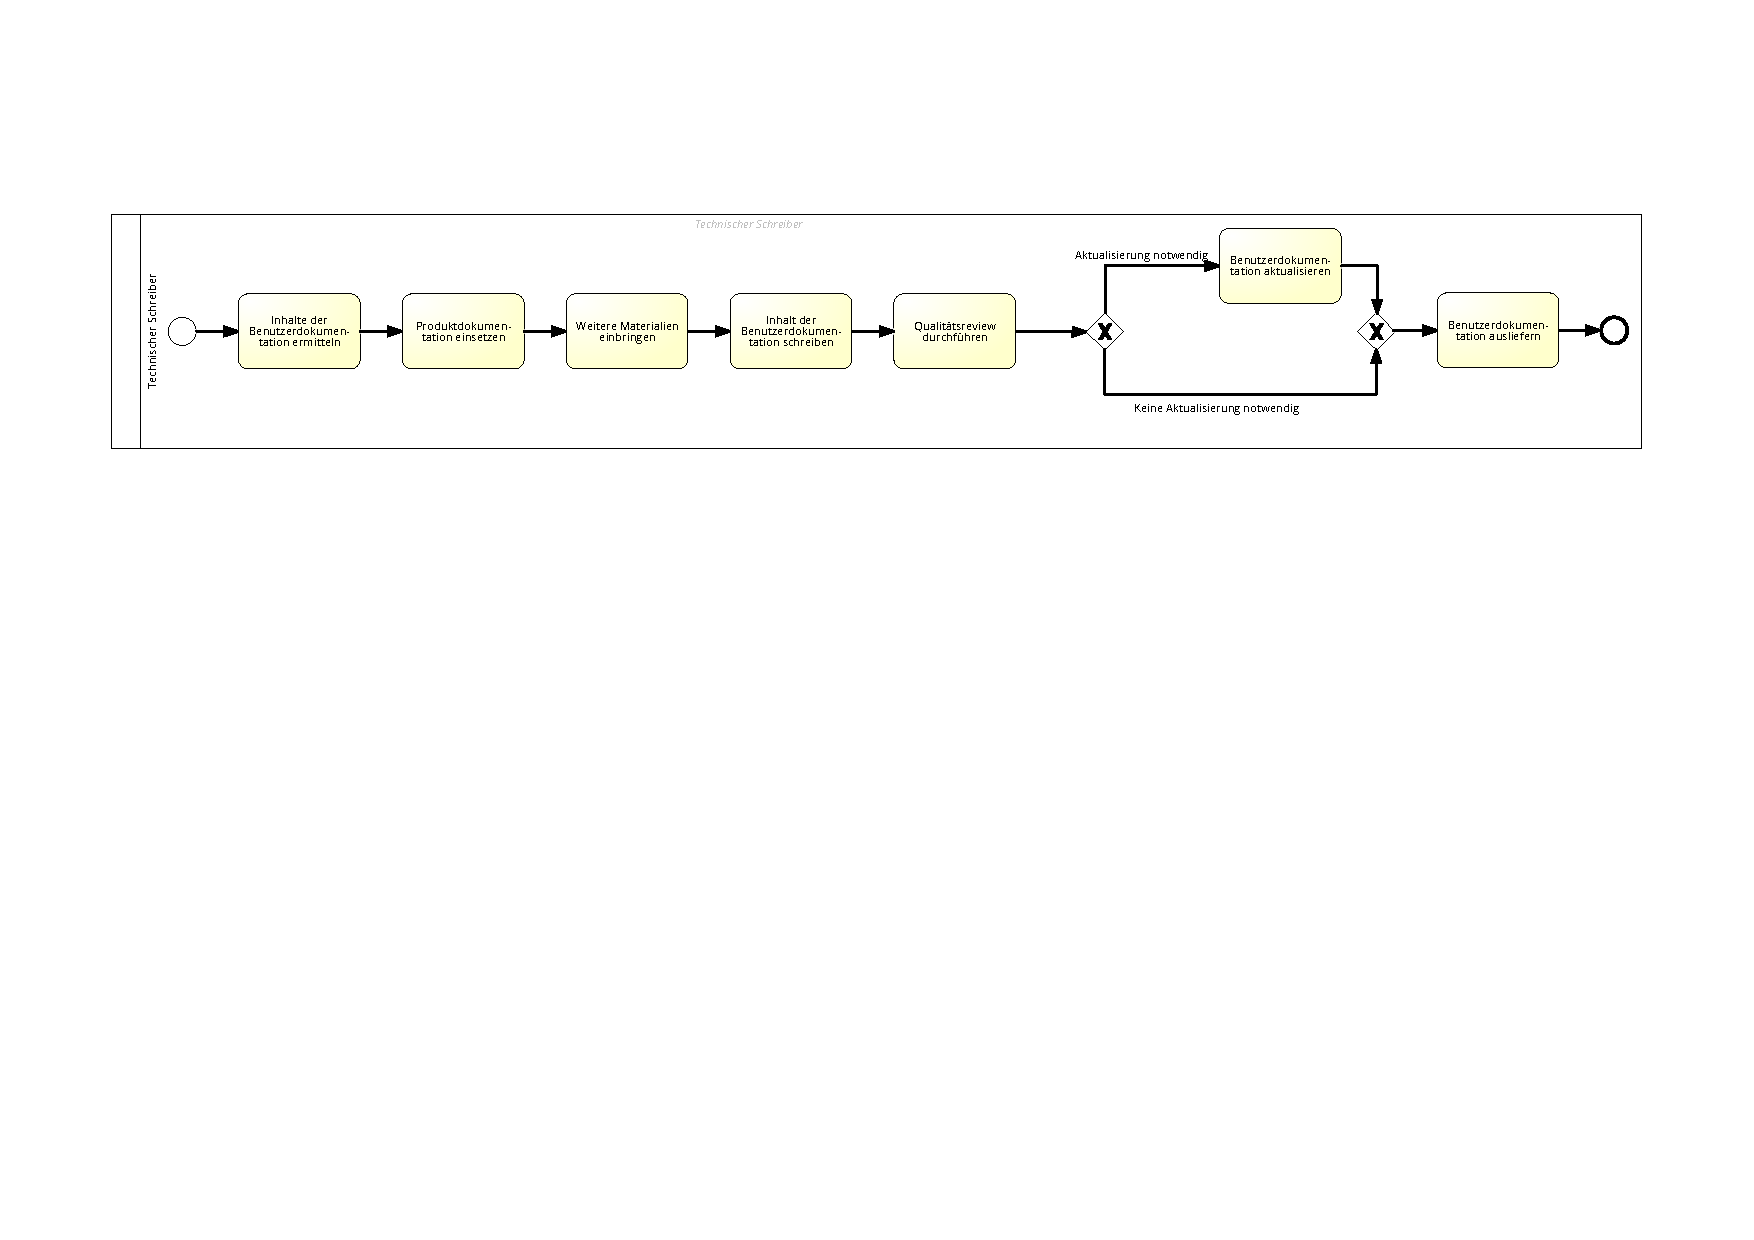
\includegraphics[width=\linewidth]{BenutzerDokumentationErstellen} %pdf, jpg, png...
  \caption{Develop Product Documentation-Construction Unterprozess BenutzerdokumentationErstellen}
  \label{fig:BenutzerDokumentationErstellen}
\end{center}
\end{figure}


\begin{figure}[htp]
\begin{center}
  \includegraphics[width=\linewidth]{UnterstuetzungsDokumentationErstellen} %pdf, jpg, png...
  \caption{Develop Product Documentation-Construction Unterprozess UnterstützungsdokumentationErstellen}
  \label{fig:UnterstuetzungsdokumentationErstellen}
\end{center}
\end{figure}

\begin{figure}[htp]
\begin{center}
  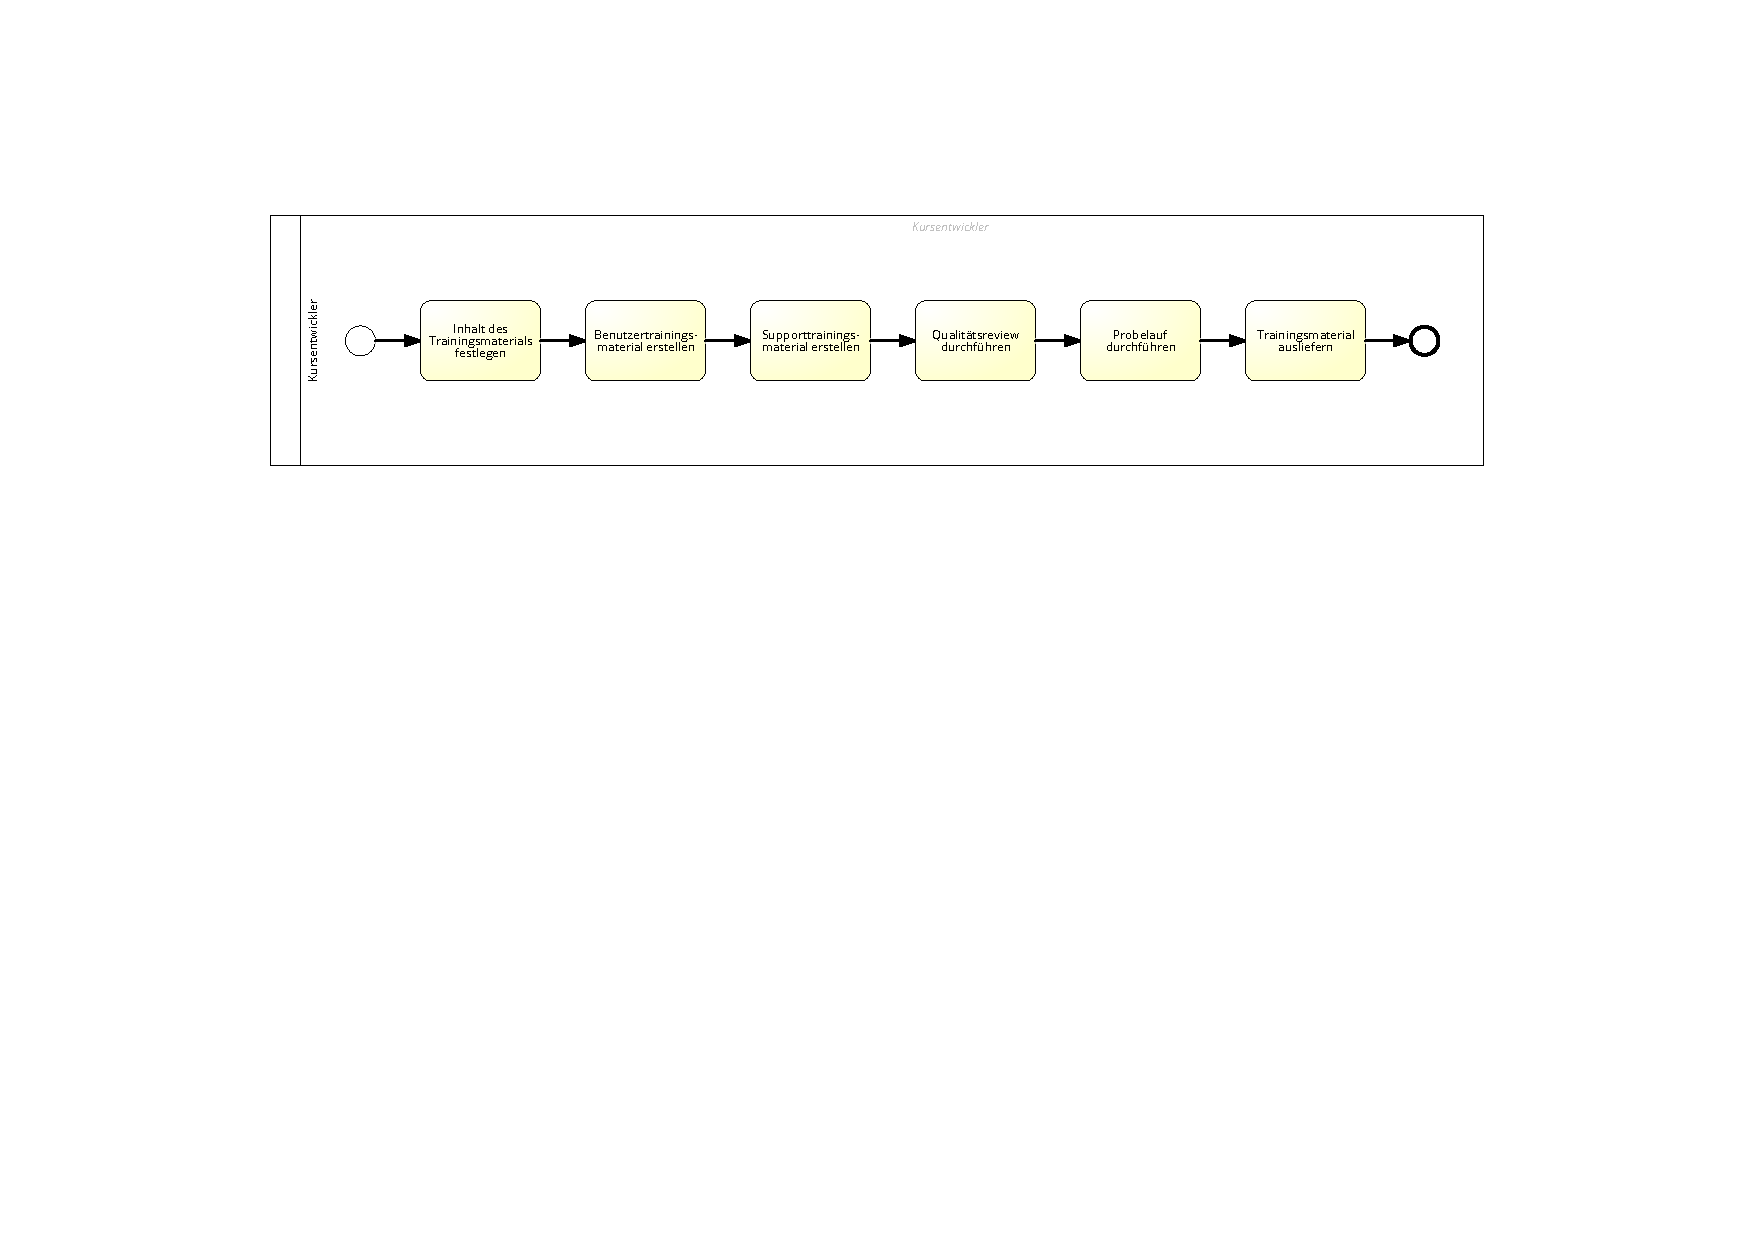
\includegraphics[width=\linewidth]{TrainingsmaterialErstellen} %pdf, jpg, png...
  \caption{Develop Product Documentation-Construction Unterprozess Trainingsmaterial erstellen}
  \label{fig:TrainingsmaterialErstellen}
\end{center}
\end{figure}

\subsection{Deklarative Modellierung Open Up}


\begin{figure}[htp]
\begin{center}
  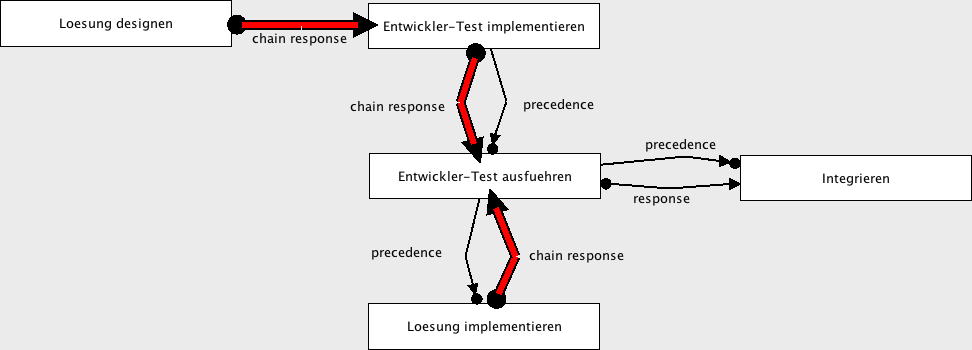
\includegraphics[width=\linewidth]{DevelopSolutionIncrement} %pdf, jpg, png...
  \caption{Develop Solution Increment deklarativ}
  \label{fig:Develop}
\end{center}
\end{figure}

\begin{figure}[htp]
\begin{center}
  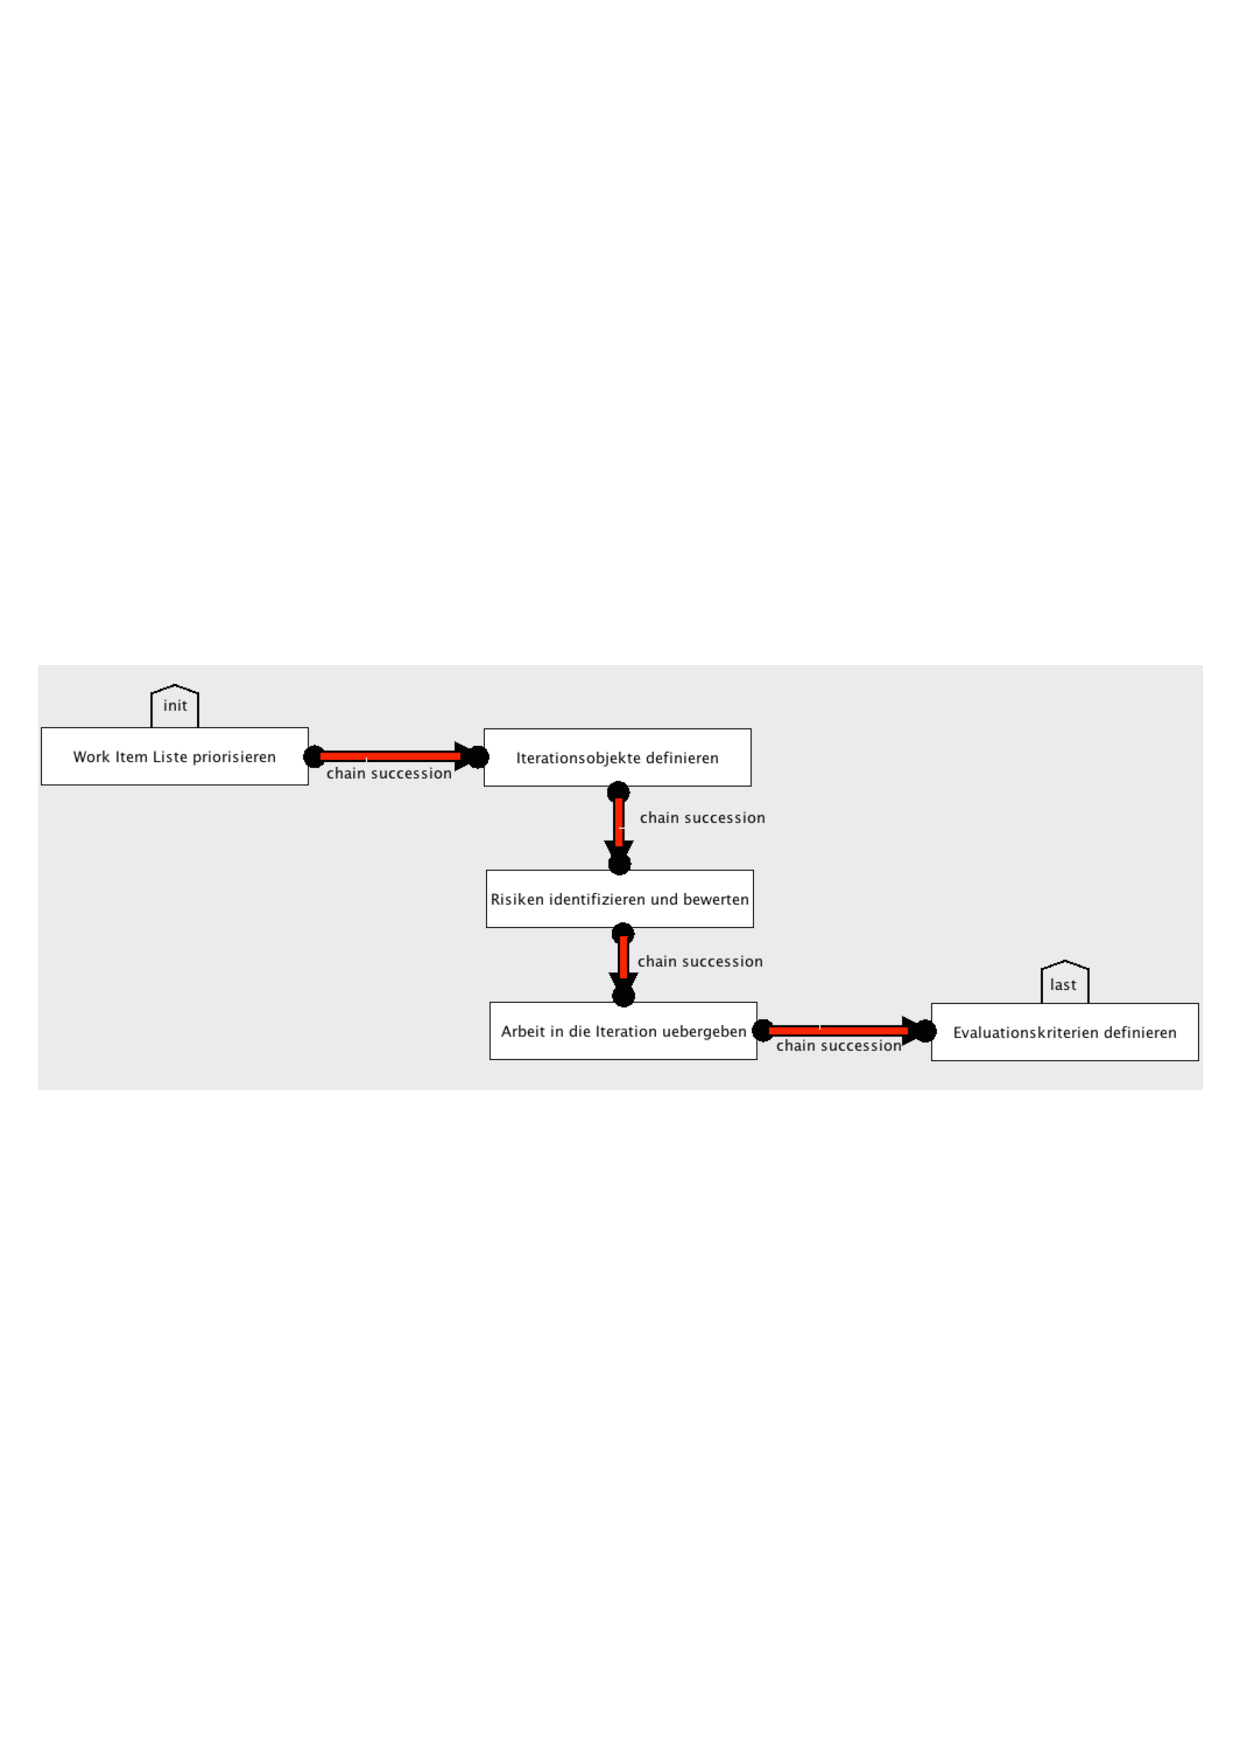
\includegraphics[width=\linewidth]{PlanIterationdeclare} %pdf, jpg, png...
  \caption{Plan and manage iteration deklarativ}
  \label{fig:PlanIterationdeclare}
\end{center}
\end{figure}
\subsection{Vergleich}







\section{V-Modell XT}


Das V-Modell XT zählt zu den schwergewichtigen Prozessmodellen \cite{Hanser2010}. Es wird als Entwicklungsstandard für die Durchführung von IT-Vorhaben in der öffentlichen Verwaltung in Deutschland herangezogen \cite{Kuhrmann2011}. Beschrieben werden im V-Modell XT die Abläufe im Verlauf eines Entwicklungsprojektes über Produkte, Rollen und Aktivitäten \cite{Friedrich2008}. Es wird somit ganz genau geregelt, \textit{Wer}, \textit{Wann}, \textit{Was} in einem Projekt zu tun hat \cite{2004vmodell}. Die Vorgehensbausteine ermöglichen neben einer Modularisierung der Abläufe auch eine flexible Zusammenstellung, wodurch das V-Modell XT auf die jeweils eigene Situation angepasst werden kann. \cite{Friedrich2008,Zoerner2012}. \newline
\subsection{Analyse V-Modell XT}

Abbildung \ref{fig:grundstruktur} zeigt die Grundstruktur des V-Modell XT, welche im Folgenden detailliert erläutert wird.
\begin{figure}[htp]
\begin{center}
  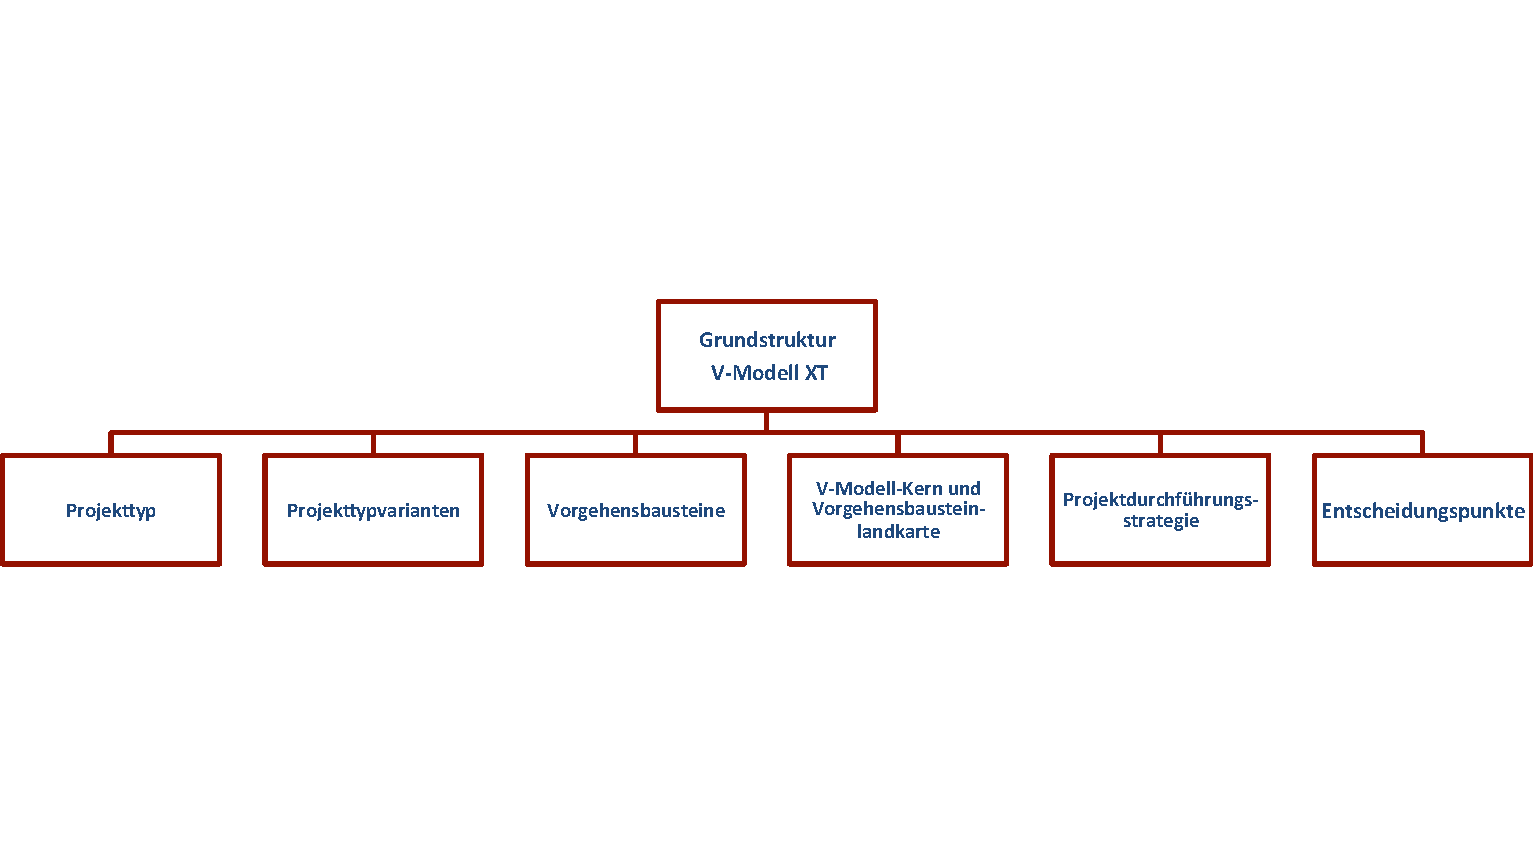
\includegraphics[width=\linewidth]{grundstruktur} %pdf, jpg, png...
  \caption{Grundstruktur V-Modell XT nach \cite{2004vmodell}}
  \label{fig:grundstruktur}
\end{center}
\end{figure}

\subsubsection{Projekttypen}
Nicht alle V-Modell-Projekttypen laufen nach exakt demselben Schema ab. Auf Grund ihrer charakteristischen Eigenschaften lassen sie sich demnach in unterschiedliche Projekttypen einteilen. Abbildung \ref{fig:Projekttypen} gibt einen ersten Überblick über die verschiedenen Projekttypen im V-Modell XT \cite{2004vmodell}.
\begin{figure}[htp]
\begin{center}
  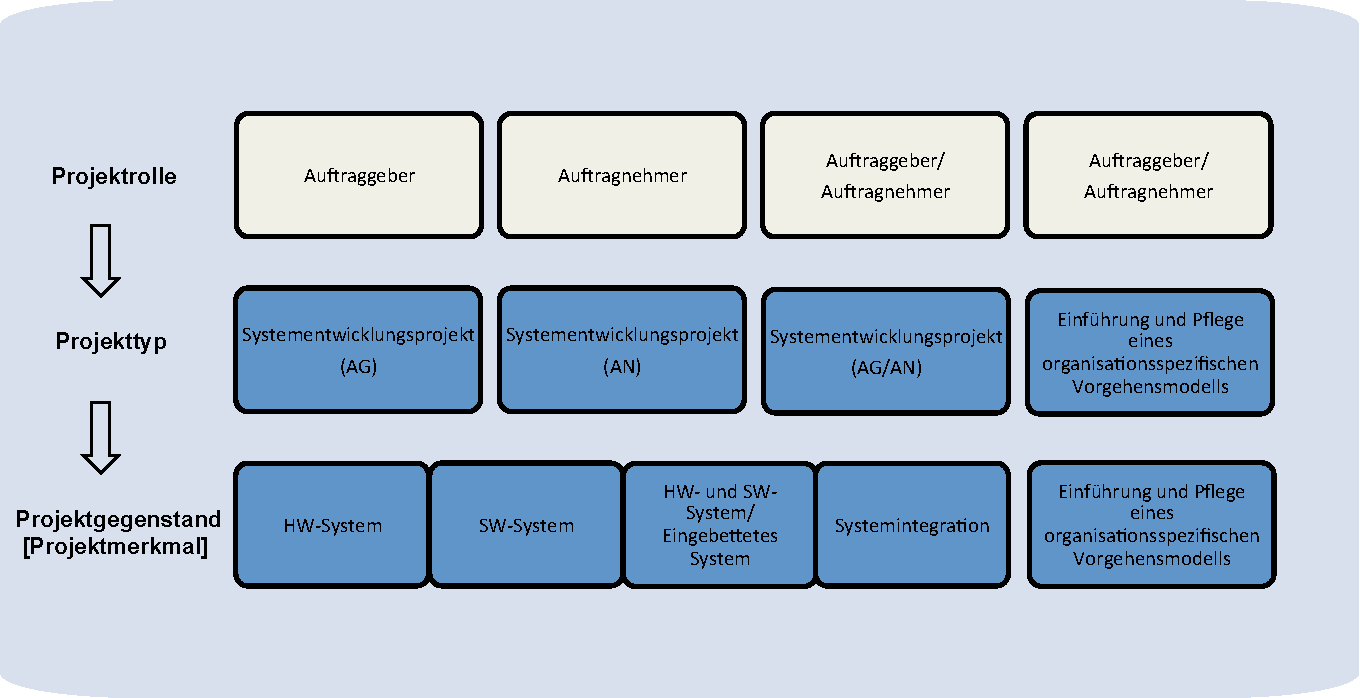
\includegraphics[width=\linewidth]{v-modell-rollen} %pdf, jpg, png...
  \caption{Projekttypen V-Modell XT nach \cite{2004vmodell}}
  \label{fig:Projekttypen}
\end{center}
\end{figure}

Es existieren somit drei verschiedene Projekttypen: \textit{Systementwicklungsprojekt eines Auftraggebers}, \textit{Systementwicklungsprojekt eines Auftragnehmers} und \textit{Einführung und Pflege eines organisationsspezifischen Vorgehensmodells} \cite{reinhard2008}. \newline

Es werden drei verschiedene Projektrollen unterschieden, welche dem jeweiligen Projekttyp entsprechen: In der Rolle \textit{Auftragnehmer} wird ein vom \textit{Auftraggeber} spezifiziertes System entwickelt. Die Systementwicklung wird an einen oder mehrere \textit{Arbeitnehmer} weiter gegeben, wenn man sich in der Rolle \textit{Arbeitgeber} befindet. Das System  wird selbst entwickelt in der Rolle \textit{Auftraggeber/Auftragnehmer} \cite{brack2010,2004vmodell}.\newline


Beim \textit{Systementwicklungsprojekt eines Auftraggebers} wird die Entwicklung des Projektgegenstandes im Projektverlauf  ausgeschrieben und der Auftragnehmer trifft eine Auswahl anhand der eingehenden Angebote. Der Auftragnehmer, welcher für die Entwicklung des Projektgegenstandes ausgewählt wurde, entwickelt den Projektgegenstand, welcher dann vom Auftragnehmer abgenommen wird \cite{reinhard2008,2004vmodell}.\newline
Umgekehrt wird beim \textit{Systementwicklungsprojekt eines Auftragnehmers} im Laufe des Projektes ein Angebot erstellt und bei Auswahl durch den Auftraggeber ein Projektgegenstand entwickelt, welcher abschließend an den Auftraggeber ausgeliefert und von diesem abgenommen wird \cite{reinhard2008,2004vmodell}.\newline
Bei \textit{Einführung und Pflege eines organisationsspezifischen Vorgehensmodells} geht es um Projekte, welche Prozessmodelle z.B. das V-Modell einführen und verbessern wollen. Für diesen Zweck ist eine Analyse des vorherigen Prozessmodelles notwendig und etwaige Verbesserungsmöglichkeiten sind zu erfassen und durchzuführen \cite{reinhard2008,2004vmodell}.\newline
Wie aus Abbildung \ref{fig:Projekttypen} ersichtlich ist, kann es sich im V-Modell XT beim Projektgegenstand um ein Hardware (HW)-System, ein Software (SW)-System, ein eingebettetes System oder eine Systemintegration handeln \cite{brack2010,2004vmodell}. \newline

\subsubsection{Projekttypvarianten}
Für jeden der Projekttypen, gibt es im V-Modell XT mindestens eine passende Projekttypvariante. Diese bestimmt die Rahmenbedingungen für mögliche Abläufe eines Projektes. In Abbildung \ref{fig:Projekttypen} sind die verschiedenen Projekttypvarianten des V-Modell XT aufgelistet und es wird gezeigt, mit welchen Merkmalen die zugehörigen Projekttypvarianten ausgewählt werden können \cite{2004vmodell}.   
\begin{figure}[htp]
\begin{center}
  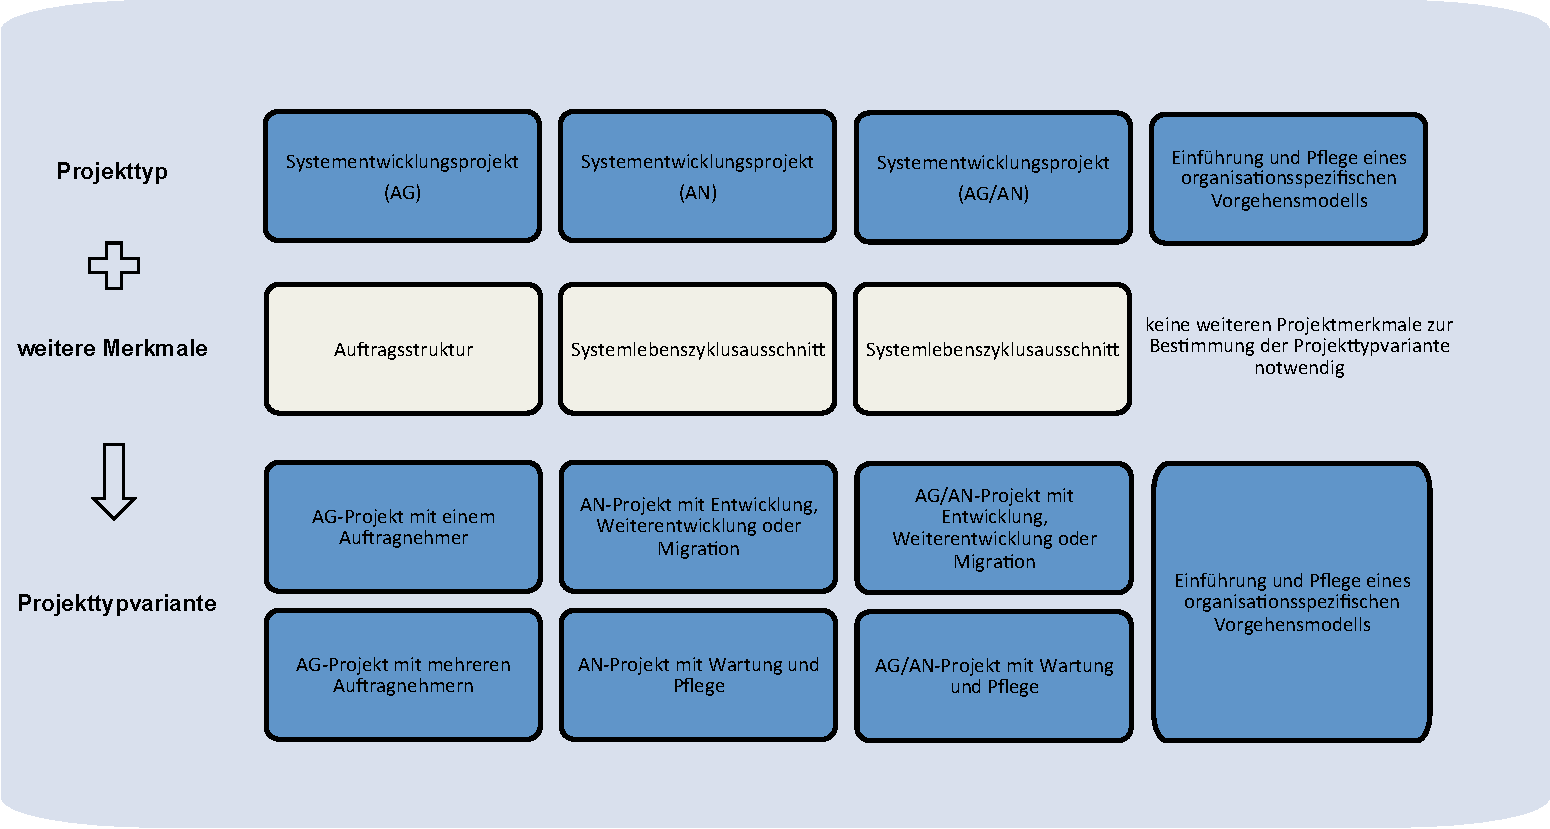
\includegraphics[width=\linewidth]{Projekttypvarianten-v-modell} %pdf, jpg, png...
  \caption{Zuordnung der Projekttypvarianten zu den Projekttypen des V-Modell XT \cite{2004vmodell}}
  \label{fig:Projekttypen}
\end{center}
\end{figure}
 Hieraus ist ersichtlich, dass für den Projekttyp \textit{Einführung und Pflege eines organisationsspezifischen Vorgehensmodells} nur eine einzige Projekttypvariante existiert \cite{2004vmodell}.\newline
Für den Projekttyp \textit{Systementwicklungsprojekt (AG)} existieren zwei verschiedene Projekttypvarianten. Falls der Auftraggeber mit nur einem Auftragnehmer zusammen arbeitet, ergibt sich die Projekttypvariante \textit{Systementwicklungsprojekt (AG)- Projekt mit einem Auftragnehmer}. Arbeitet der Auftraggeber mit mehreren Auftragnehmern zusammen ergibt sich die Projekttypvariante \textit{Systementwicklungsprojekt (AG)- Projekt mit mehreren Auftragnehmern}\cite{2004vmodell}.\newline
Bei den Projekttypen \textit{Systementwicklungsprojekt (AN)} und \textit{Systementwicklungsprojekt (AG/AN)} wird die Unterscheidung anhand des Systemlebenszyklusausschnitt des Projektes durchgeführt. Somit in wird den Systemlebenszyklusausschnitten Entwicklung, Weiterentwicklung und Migration eine andere Projekttypvariante gewählt, als in Wartung und Pflege \cite{2004vmodell}.\newline 
  
 \subsubsection{Vorgehensbausteine}
Modulare, aufeinander aufbauende Vorgehensbausteine bilden den Kern des V-Modell XT. Vorgehensbausteine sind selbständig entwickelbare und änderbare Einheiten und bestehen aus Aktivitäten, Produkten und Rollen. Sie geben einerseits vor, \grqq Was\grqq{}  in einem Projekt zu tun ist, also welche Produkte zu erstellen sind und andererseits \grqq Wer\grqq, also welche konkrete Rolle für das jeweilige Produkt verantwortlich ist. Abbildung \ref{fig:vorgehensbausteine} gibt einen Überblick über diese \cite{ruf2008, 2004vmodell}.\newline

\begin{figure}[htp]
\begin{center}
  \includegraphics[width=\linewidth]{vorgehensbaustein} %pdf, jpg, png...
  \caption{Vorgehensbausteine V-Modell XT nach \cite{2004vmodell}}
  \label{fig:vorgehensbausteine}
\end{center}
\end{figure}

Ergebnisse und Zwischenergebnisse werden Produkte genannt. Komplexe Produkte können in ein oder mehrere Themen gegliedert werden und inhaltlich zusammengehörende Produkte können zu einer Disziplin zusammengefasst werden. Produkte können hierbei auch voneinander abhängig sein, sowohl innerhalb eines Vorgehensbausteins, als auch zwischen verschiedenen Vorgehensbausteinen \cite{2004vmodell}.\newline
Jedes Produkt wird von genau einer Aktivität fertig gestellt. Aktivitäten legen auch fest, wie die einzelnen Produkte zu bearbeiten sind. Sie bestehen aus einer oder mehreren Teilaktivitäten, sogenannten Arbeitsschritten. Diese stellen eine Art Arbeitsanleitung dar und bearbeiten eine oder mehrere Themen \cite{2004vmodell}.\newline
Durch Rollen werden eine Menge von Aufgaben und Verantwortlichkeiten gekapselt, wodurch das V-Modell XT unabhängig von organisatorischen Rahmenbedingungen bleibt. Eine Zuordnung von Personen, bzw. Organisationseinheiten zu einer Rolle erfolgt erst zu Beginn eines Projektes. Es wird jedem Produkt genau eine Rolle als Verantwortlicher zugewiesen, weitere Rollen können am Produkt als Mitwirkende mitarbeiten \cite{2004vmodell}. \newline



\subsubsection{V-Modell-Kern und Vorgehensbausteinlandkarte}

Um ein spezifisches Projekt an ein V-Modell-Projekt anzupassen, ist für jeden Projekttyp und jede Projekttypvariante genau vorgegeben, welche Vorgehensbausteine jeweils anzuwenden sind \cite{2004vmodell}. Hierdurch kann also ein individuelles V-Modell für ein Projekt erstellt werden \cite{heinrich2007}. Hierfür ist es notwendig, die Vorgehensbausteine für ein V-Modell-Projekt nach den Vorgaben des Projekttyps auszuwählen und festzulegen \cite{2004vmodell}. \newline

\begin{figure}[htp]
\begin{center}
  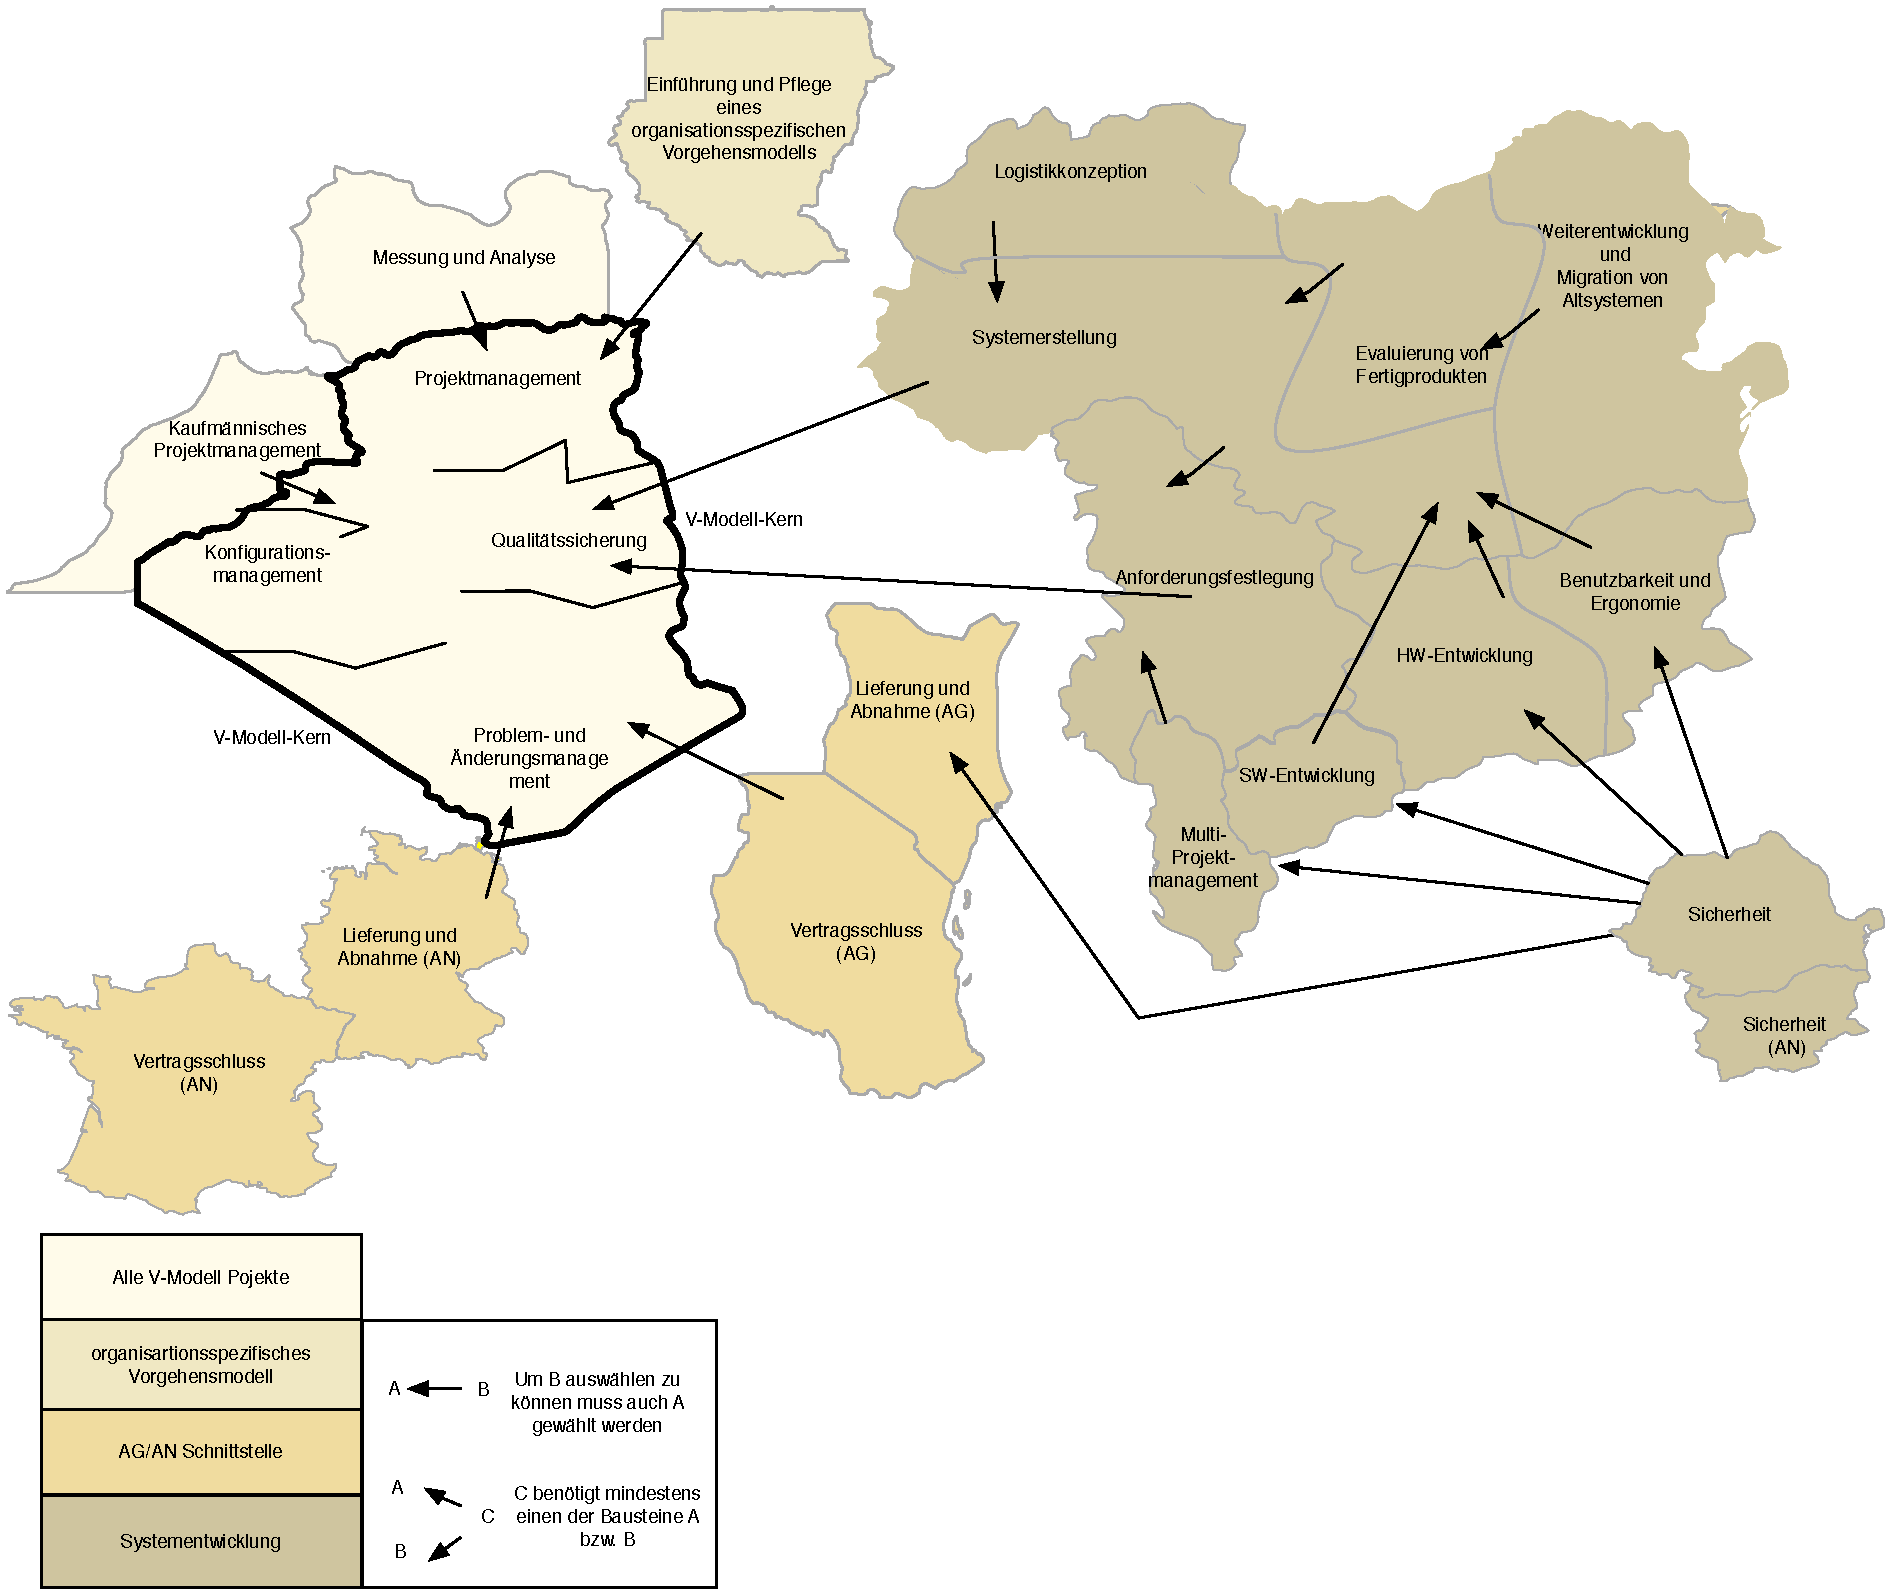
\includegraphics[width=\linewidth]{landkarte} %pdf, jpg, png...
  \caption{V-Modell-Kern und Vorgehensbausteinlandkarte nach \cite{2004vmodell}}
  \label{fig:landkarte}
\end{center}
\end{figure}

 Wie Abbildung \ref{fig:landkarte} zeigt, können die Vorgehensbausteine in die vier Bereiche \textit{Alle V-Modell-Projekte}, \textit{Organisationsspezifisches Vorgehensmodell}, \textit{AG/AN-Schnittstelle} und \textit{Systementwicklung} eingeteilt werden \cite{2004vmodell}.\newline
 Im Bereich \textit{Alle V-Modell-Projekte} finden sich diejenigen Vorgehensbausteine, welche in jedem V-Modell-Projekt herangezogen werden können. Zudem gibt es den V-Modell-Kern, in welchem sich die Vorgehensmodelle finden, die in jedem V-Modell-Projekt unerlässlich sind: \textit{Projektmanagement}, \textit{Konfigurationsmanagement}, \textit{Problem- und Änderungsmanagement} und \textit{Qualitätssicherung}. Zusätzlich zu diesen verpflichtenden Vorgehensbausteinen können in jedem Projekt noch \textit{Kaufmännisches Projektmanagement}, welches bei der Integration des Projektmanagements in das kaufmännische Management hilft und \textit{Messung und Analyse}, welches Verfahren für die organisationsweite und projektübergreifende Erfassung und Auswertung von Kennzahlen bereitstellt, verwendet werden \cite{2004vmodell}.\newline
 Ist der Zweck eines Projektes die Entwicklung eines \textit{Organisationsspezifischen Vorgehensmodells}, so muss der Vorgehensbaustein \textit{Einführung und Pflege eines organisationsspezifischen Vorgehensmodells} hinzugenommen werden. In diesem finden sich Verfahren und Richtlinien für die Einführung eines Vorgehensmodells innerhalb einer Organisation sowie die damit einhergehende Etablierung eines stetigen Verbesserungsprozesses \cite{2004vmodell}.\newline
 Wenn ein Projekt die Entwicklung eines Systems zum Ziel hat so wird der Bereich \textit{Systementwicklung} herangezogen. In diesem befinden sich die Vorgehensbausteine \textit{Anforderungsfestlegung}, \textit{Systemerstellung}, \textit{HW-Entwicklung}, \textit{SW-Entwicklung}, \textit{Logistikkonzeption}, \textit{Weiterentwicklung und Migration von Altsystemen}, \textit{Evaluierung von Fertigprodukten}, \textit{Benutzbarkeit und Ergonomie}, \textit{Sicherheit} sowie \textit{Sicherheit (AN)} und \textit{Multi-Projektmanagement} \cite{2004vmodell}. \newline
 Im Bereich \textit{AG/AN-Schnittstelle} befinden sich die Vorgehensbausteine für die Kommunikation zwischen Arbeitgeber und Arbeitnehmer: \textit{Lieferung und Abnahme (AG)}, \textit{Lieferung und Abnahme (AN)}, \textit{Vertragsschluss (AG)} und \textit{Vertragsschluss (AN)}. Hier finden sich Regelungen über den Vertrag zwischen Arbeitgeber und Arbeitnehmer sowie über Lieferung und Abnahme des Entwicklungsgegenstandes \cite{2004vmodell}. \newline
 
 \subsubsection{Projektdurchführungsstrategie}
 Die Vorgehensbausteine im V-Modell XT geben zwar an, welche Produkte jeweils zu erstellen und welche Aktivitäten durchzuführen sind, sie geben jedoch hierbei nicht vor, in welcher Reihenfolge dies geschehen soll. Damit das Projekt trotzdem geplant und gesteuert werden kann, gibt es im V-Modell eine Projektdurchführungsstrategie, welche auf den jeweiligen Projekttyp und die Projekttypvariante abgestimmt ist. Hier wird somit die Reihenfolge der Produkte und Aktivitäten festgelegt, also das  \grqq Wann\grqq {}. festgelegt. Außerdem werden hier zu erreichende Projektfortschrittsstufen vorgegeben \cite{2004vmodell}. \newline
 
 \subsubsection{Entscheidungspunkte}
Abbildung \ref{fig:entscheidungspunkte} zeigt, dass die in der Projektdurchführungsstrategie vorgegebenen Projektfortschrittsstufen bei Erreichen durch Entscheidungspunkte markiert werden, welche einen Meilenstein im Projektablauf darstellen. Um den Entscheidungspunkt zu erreichen muss eine vorgegebene Menge an Produkten fertig gestellt werden. Hier entscheidet das Projektmanagement über das Erreichen der Projektfortschrittsstufe und das Freigeben des nächsten Projektabschnitts. Die Entscheidungspunkte, welche im V-Modell XT erreicht werden müssen, können Abbildung \ref{fig:v-modell} entnommen werden. Diese werden wie im V-Modell-Kern in die vier Bereiche \textit{Alle V-Modell-Projekte}, \textit{Organisationsspezifisches Vorgehensmodell}, \textit{AG/AN-Schnittstelle} und \textit{Systementwicklung} unterschieden \cite{2004vmodell}. \newline
Demnach gelten die Entscheidungspunkte \textit{Projekt genehmigt}, \textit{Projekt definiert}, \textit{Iteration geplant} und \textit{Projekt abgeschlossen} für alle Projekttypen und Projektdurchführungsstrategien \cite{2004vmodell}. \newline
Bei der Systementwicklung werden die Entscheidungspunkte \textit{Anforderungen festgelegt}, \textit{System spezifiziert}, \textit{System entworfen}, \textit{Feinentwurf abgeschlossen}, \textit{Systemelemente realisiert} und \textit{System integriert} verwendet. Falls das Projekt vor der Anforderungserhebung in mehrere Teilmodelle aufgeteilt werden soll, werden zusätzlich die Entscheidungspunkte \textit{Gesamtprojekt aufgeteilt} und \textit{Gesamtprojektfortschritt überprüft} hinzugenommen \cite{2004vmodell}. \newline
Die Entscheidungspunkte für die Arbeitgeber/Arbeitnehmer Schnittstelle setzen sich aus \textit{Projekt ausgeschrieben}, \textit{Angebot abgegeben}, \textit{Projekt beauftragt}, \textit{Lieferung durchgeführt}, \textit{Abnahme erfolgt} und \textit{Projektfortschritt überprüft} zusammen \cite{2004vmodell}. \newline
 Bei der Entwicklung eines organisationsspezifischen Vorgehensmodells kommen die Entscheidungspunkte \textit{Vorgehensmodell analysiert}, \textit{Verbesserung Vorgehensmodell konzipiert} und \textit{Verbesserung Vorgehensmodell realisiert} zum Einsatz \cite{2004vmodell}. \newline
 Die Entscheidungspunkte legen das \grqq Wann\grqq {} und \grqq Was\grqq {} fest, d.h. wann welche Produkte fertig gestellt sein müssen.

 
 
 \begin{figure}[htp]
\begin{center}
  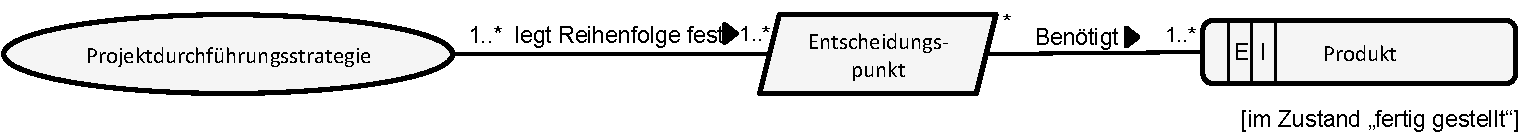
\includegraphics[width=\linewidth]{Entscheidungspunkte} %pdf, jpg, png...
  \caption{Entscheidungspunkte V-Modell XT nach \cite{2004vmodell}}
  \label{fig:entscheidungspunkte}
\end{center}
\end{figure}
 
\begin{sidewaysfigure}[htp]
\begin{center}
  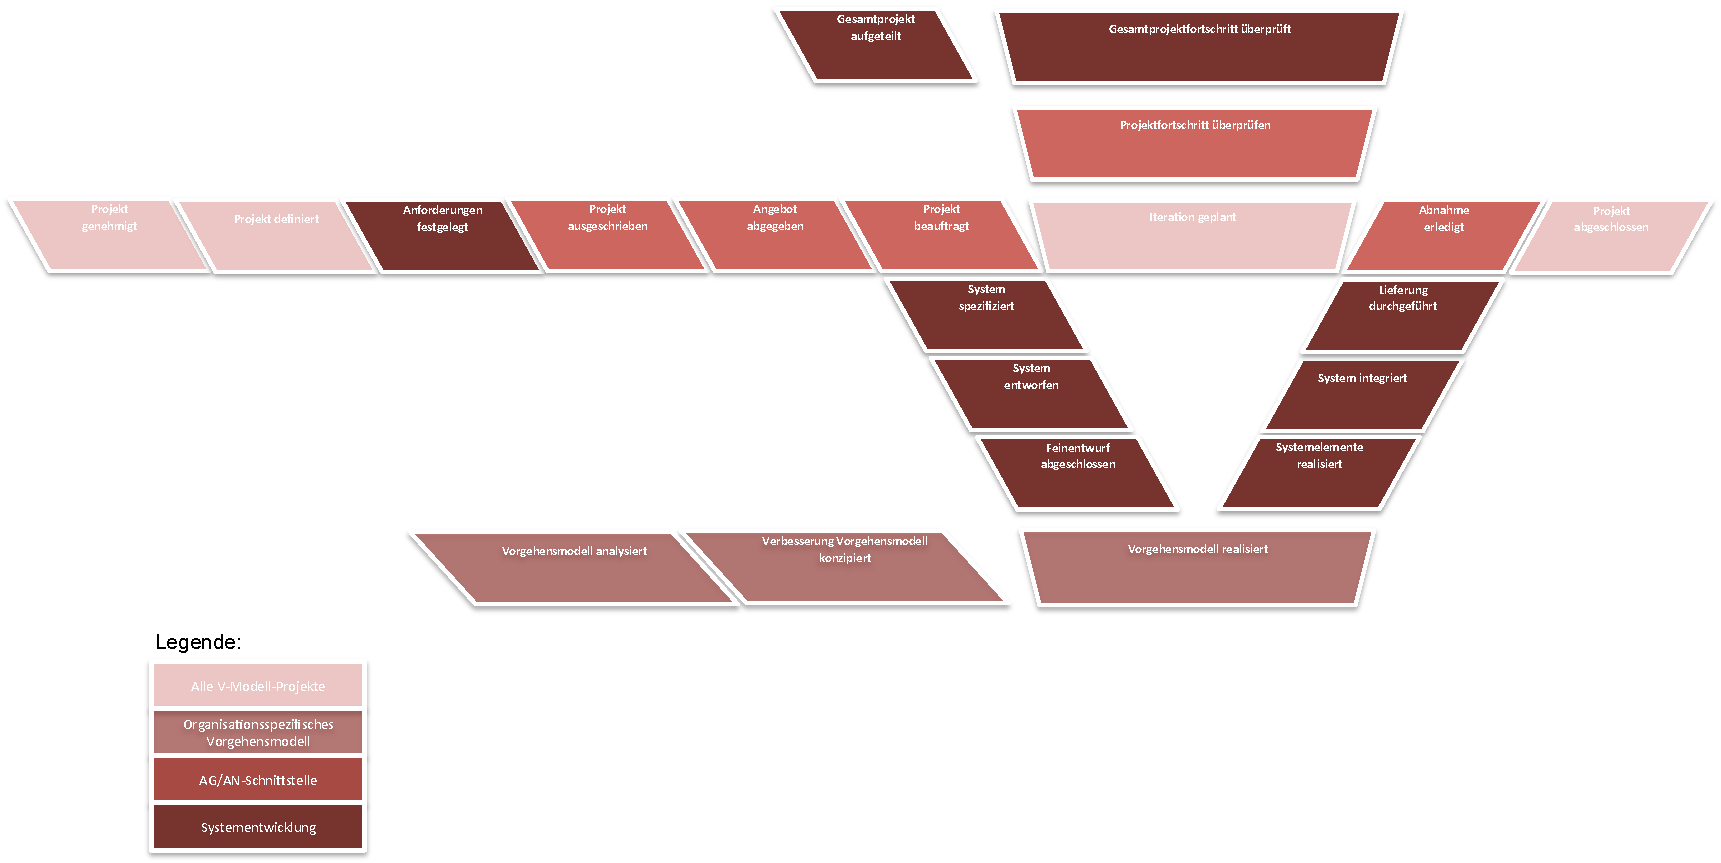
\includegraphics[scale=0.7]{v-modell} %pdf, jpg, png...
  \caption{Entscheidungspunkte für die Projektdurchführungsstrategie nach \cite{2004vmodell}}
  \label{fig:v-modell}
\end{center}
\end{sidewaysfigure}
\subsection{Imperative Modellierung V-Modell}
\subsection{Deklarative Modellierung V-Modell}
\subsection{Vergleich}



